% Copyright © 2013 Martin Ueding <dev@martin-ueding.de>

% Copyright © 2012-2013 Martin Ueding <dev@martin-ueding.de>

% This is my general purpose LaTeX header file for writing German documents.
% Ideally, you include this using a simple ``% Copyright © 2012-2013 Martin Ueding <dev@martin-ueding.de>

% This is my general purpose LaTeX header file for writing German documents.
% Ideally, you include this using a simple ``% Copyright © 2012-2013 Martin Ueding <dev@martin-ueding.de>

% This is my general purpose LaTeX header file for writing German documents.
% Ideally, you include this using a simple ``\input{header.tex}`` in your main
% document and start with ``\title`` and ``\begin{document}`` afterwards.

% If you need to add additional packages, I recommend not doing this in this
% file, but in your main document. That way, you can just drop in a new
% ``header.tex`` and get all the new commands without having to merge manually.

% Since this file encorporates a CC-BY-SA fragment, this whole files is
% licensed under the CC-BY-SA license.

\documentclass[11pt, ngerman, fleqn, DIV=15, BCOR=2cm, headinclude]{scrartcl}

\usepackage{graphicx}

% Environment to quote the problem. Currently, this is just a new name for the
% quote environment.
\newenvironment{problem}{\begin{quote}\textsf{\textbf{Aufgabenstellung:}}\quad}{\end{quote}}

\setkomafont{caption}{\sf}
\setkomafont{captionlabel}{\usekomafont{caption}}

%%%%%%%%%%%%%%%%%%%%%%%%%%%%%%%%%%%%%%%%%%%%%%%%%%%%%%%%%%%%%%%%%%%%%%%%%%%%%%%
%                                Locale, date                                 %
%%%%%%%%%%%%%%%%%%%%%%%%%%%%%%%%%%%%%%%%%%%%%%%%%%%%%%%%%%%%%%%%%%%%%%%%%%%%%%%

\usepackage{babel}
\usepackage[iso]{isodate}

%%%%%%%%%%%%%%%%%%%%%%%%%%%%%%%%%%%%%%%%%%%%%%%%%%%%%%%%%%%%%%%%%%%%%%%%%%%%%%%
%                          Margins and other spacing                          %
%%%%%%%%%%%%%%%%%%%%%%%%%%%%%%%%%%%%%%%%%%%%%%%%%%%%%%%%%%%%%%%%%%%%%%%%%%%%%%%

\usepackage[parfill]{parskip}
\usepackage{setspace}
\usepackage[activate]{microtype}

\setlength{\columnsep}{2cm}

%%%%%%%%%%%%%%%%%%%%%%%%%%%%%%%%%%%%%%%%%%%%%%%%%%%%%%%%%%%%%%%%%%%%%%%%%%%%%%%
%                                    Color                                    %
%%%%%%%%%%%%%%%%%%%%%%%%%%%%%%%%%%%%%%%%%%%%%%%%%%%%%%%%%%%%%%%%%%%%%%%%%%%%%%%

\usepackage[usenames, dvipsnames]{xcolor}

\colorlet{darkred}{red!70!black}
\colorlet{darkblue}{blue!70!black}
\colorlet{darkgreen}{green!40!black}

%%%%%%%%%%%%%%%%%%%%%%%%%%%%%%%%%%%%%%%%%%%%%%%%%%%%%%%%%%%%%%%%%%%%%%%%%%%%%%%
%                         Font and font like settings                         %
%%%%%%%%%%%%%%%%%%%%%%%%%%%%%%%%%%%%%%%%%%%%%%%%%%%%%%%%%%%%%%%%%%%%%%%%%%%%%%%

% This replaces all fonts with Bitstream Charter, Bitstream Vera Sans and
% Bitstream Vera Mono. Math will be rendered in Charter.
\usepackage[charter, greekuppercase=italicized]{mathdesign}
\usepackage{beramono}
\usepackage{berasans}

% Bold, sans-serif tensors. This fragment is taken from “egreg” from
% http://tex.stackexchange.com/a/82747/8945 and licensed under `CC-BY-SA
% <https://creativecommons.org/licenses/by-sa/3.0/>`_.
\usepackage{bm}
\DeclareMathAlphabet{\mathsfit}{\encodingdefault}{\sfdefault}{m}{sl}
\SetMathAlphabet{\mathsfit}{bold}{\encodingdefault}{\sfdefault}{bx}{sl}
\newcommand{\tens}[1]{\bm{\mathsfit{#1}}}

% Bold vectors.
\renewcommand{\vec}[1]{\boldsymbol{#1}}

%%%%%%%%%%%%%%%%%%%%%%%%%%%%%%%%%%%%%%%%%%%%%%%%%%%%%%%%%%%%%%%%%%%%%%%%%%%%%%%
%                               Input encoding                                %
%%%%%%%%%%%%%%%%%%%%%%%%%%%%%%%%%%%%%%%%%%%%%%%%%%%%%%%%%%%%%%%%%%%%%%%%%%%%%%%

\usepackage[T1]{fontenc}
\usepackage[utf8]{inputenc}

%%%%%%%%%%%%%%%%%%%%%%%%%%%%%%%%%%%%%%%%%%%%%%%%%%%%%%%%%%%%%%%%%%%%%%%%%%%%%%%
%                         Hyperrefs and PDF metadata                          %
%%%%%%%%%%%%%%%%%%%%%%%%%%%%%%%%%%%%%%%%%%%%%%%%%%%%%%%%%%%%%%%%%%%%%%%%%%%%%%%

\usepackage{hyperref}
\usepackage{lastpage}

% This sets the author in the properties of the PDF as well. If you want to
% change it, just override it with another ``\hypersetup`` call.
\hypersetup{
	breaklinks=false,
	citecolor=darkgreen,
	colorlinks=true,
	linkcolor=darkblue,
	menucolor=black,
	pdfauthor={Martin Ueding},
	urlcolor=darkblue,
}

%%%%%%%%%%%%%%%%%%%%%%%%%%%%%%%%%%%%%%%%%%%%%%%%%%%%%%%%%%%%%%%%%%%%%%%%%%%%%%%
%                               Math Operators                                %
%%%%%%%%%%%%%%%%%%%%%%%%%%%%%%%%%%%%%%%%%%%%%%%%%%%%%%%%%%%%%%%%%%%%%%%%%%%%%%%

% AMS environments like ``align`` and theorems like ``proof``.
\usepackage{amsmath}
\usepackage{amsthm}

% Common math constructs like partial derivatives.
\usepackage{commath}

% Physical units.
\usepackage[output-decimal-marker={,}]{siunitx}

% Since I use mathdesign with italic uppercase greek characters, the Ohm unit will be displayed with an italic Ω by default. Units have to be roman, so this forces it the right way.
\DeclareSIUnit{\ohm}{$\Omegaup$}
\DeclareSIUnit{\division}{DIV}
\DeclareSIUnit{\voltss}{$\mathrm{V_{SS}}$}

% Word like operators.
\DeclareMathOperator{\acosh}{arcosh}
\DeclareMathOperator{\arcosh}{arcosh}
\DeclareMathOperator{\arcsinh}{arsinh}
\DeclareMathOperator{\arsinh}{arsinh}
\DeclareMathOperator{\asinh}{arsinh}
\DeclareMathOperator{\card}{card}
\DeclareMathOperator{\csch}{cshs}
\DeclareMathOperator{\diam}{diam}
\DeclareMathOperator{\sech}{sech}
\renewcommand{\Im}{\mathop{{}\mathrm{Im}}\nolimits}
\renewcommand{\Re}{\mathop{{}\mathrm{Re}}\nolimits}

% Fourier transform.
\DeclareMathOperator{\fourier}{\ensuremath{\mathcal{F}}}

% Roman versions of “e” and “i” to serve as Euler's number and the imaginary
% constant.
\newcommand{\ee}{\eup}
\newcommand{\eup}{\mathrm e}
\newcommand{\ii}{\iup}
\newcommand{\iup}{\mathrm i}

% Symbols for the various mathematical fields (natural numbers, integers,
% rational numbers, real numbers, complex numbers).
\newcommand{\C}{\ensuremath{\mathbb C}}
\newcommand{\N}{\ensuremath{\mathbb N}}
\newcommand{\Q}{\ensuremath{\mathbb Q}}
\newcommand{\R}{\ensuremath{\mathbb R}}
\newcommand{\Z}{\ensuremath{\mathbb Z}}

% Shape like operators.
\DeclareMathOperator{\dalambert}{\Box}
\DeclareMathOperator{\laplace}{\bigtriangleup}
\newcommand{\curl}{\vnabla \times}
\newcommand{\divergence}[1]{\inner{\vnabla}{#1}}
\newcommand{\vnabla}{\vec \nabla}

\newcommand{\half}{\frac 12}

% Unit vector (German „Einheitsvektor“).
\newcommand{\ev}{\hat{\vec e}}

% Scientific notation for large numbers.
\newcommand{\e}[1]{\cdot 10^{#1}}

% Mathematician's notation for the inner (scalar, dot) product.
\newcommand{\bracket}[1]{\left\langle #1 \right\rangle}
\newcommand{\inner}[2]{\bracket{#1, #2}}

% Placeholders.
\newcommand{\emesswert}{\del{\messwert \pm \messwert}}
\newcommand{\fehlt}{\textcolor{darkred}{Hier fehlen noch Inhalte.}}
\newcommand{\messwert}{\textcolor{blue}{\square}}
\newcommand{\punkte}{\phantom{xxxxx}}
\newcommand{\punktevon}[1]{\begin{flushright}/ #1\end{flushright}}

% Separator for equations on a single line.
\newcommand{\eqnsep}{,\quad}

% Quantum Mechanics
\usepackage{braket}

%%%%%%%%%%%%%%%%%%%%%%%%%%%%%%%%%%%%%%%%%%%%%%%%%%%%%%%%%%%%%%%%%%%%%%%%%%%%%%%
%                                  Headings                                   %
%%%%%%%%%%%%%%%%%%%%%%%%%%%%%%%%%%%%%%%%%%%%%%%%%%%%%%%%%%%%%%%%%%%%%%%%%%%%%%%

% This will set fancy headings to the top of the page. The page number will be
% accompanied by the total number of pages. That way, you will know if any page
% is missing.
%
% If you do not want this for your document, you can just use
% ``\pagestyle{plain}``.

\usepackage{scrpage2}

\pagestyle{scrheadings}
\automark{section}
\cfoot{\footnotesize{Seite \thepage\ / \pageref{LastPage}}}
\chead{}
\ihead{}
\ohead{\rightmark}
\setheadsepline{.4pt}

%%%%%%%%%%%%%%%%%%%%%%%%%%%%%%%%%%%%%%%%%%%%%%%%%%%%%%%%%%%%%%%%%%%%%%%%%%%%%%%
%                            Bibliography (BibTeX)                            %
%%%%%%%%%%%%%%%%%%%%%%%%%%%%%%%%%%%%%%%%%%%%%%%%%%%%%%%%%%%%%%%%%%%%%%%%%%%%%%%

\newcommand{\bibliographyfile}{../../central-bibtex/Central}
\bibliographystyle{apalike2}

%%%%%%%%%%%%%%%%%%%%%%%%%%%%%%%%%%%%%%%%%%%%%%%%%%%%%%%%%%%%%%%%%%%%%%%%%%%%%%%
%                                Abbreviations                                %
%%%%%%%%%%%%%%%%%%%%%%%%%%%%%%%%%%%%%%%%%%%%%%%%%%%%%%%%%%%%%%%%%%%%%%%%%%%%%%%

\newcommand{\dhabk}{\mbox{d.\,h.}}

%%%%%%%%%%%%%%%%%%%%%%%%%%%%%%%%%%%%%%%%%%%%%%%%%%%%%%%%%%%%%%%%%%%%%%%%%%%%%%%
%                                  Licences                                   %
%%%%%%%%%%%%%%%%%%%%%%%%%%%%%%%%%%%%%%%%%%%%%%%%%%%%%%%%%%%%%%%%%%%%%%%%%%%%%%%

\usepackage{ccicons}

\newcommand{\ccbysadetext}{%
	\begin{small}
		Dieses Werk bzw. Inhalt steht unter einer
		\href{http://creativecommons.org/licenses/by-sa/3.0/deed.de}{%
			Creative Commons Namensnennung - Weitergabe unter gleichen
		Bedingungen 3.0 Unported Lizenz}.
	\end{small}
}

\newcommand{\ccbysadetitle}{%
	Lizenz: \href{http://creativecommons.org/licenses/by-sa/3.0/deed.de}
	{CC-BY-SA 3.0 \ccbysa}
}
`` in your main
% document and start with ``\title`` and ``\begin{document}`` afterwards.

% If you need to add additional packages, I recommend not doing this in this
% file, but in your main document. That way, you can just drop in a new
% ``header.tex`` and get all the new commands without having to merge manually.

% Since this file encorporates a CC-BY-SA fragment, this whole files is
% licensed under the CC-BY-SA license.

\documentclass[11pt, ngerman, fleqn, DIV=15, BCOR=2cm, headinclude]{scrartcl}

\usepackage{graphicx}

% Environment to quote the problem. Currently, this is just a new name for the
% quote environment.
\newenvironment{problem}{\begin{quote}\textsf{\textbf{Aufgabenstellung:}}\quad}{\end{quote}}

\setkomafont{caption}{\sf}
\setkomafont{captionlabel}{\usekomafont{caption}}

%%%%%%%%%%%%%%%%%%%%%%%%%%%%%%%%%%%%%%%%%%%%%%%%%%%%%%%%%%%%%%%%%%%%%%%%%%%%%%%
%                                Locale, date                                 %
%%%%%%%%%%%%%%%%%%%%%%%%%%%%%%%%%%%%%%%%%%%%%%%%%%%%%%%%%%%%%%%%%%%%%%%%%%%%%%%

\usepackage{babel}
\usepackage[iso]{isodate}

%%%%%%%%%%%%%%%%%%%%%%%%%%%%%%%%%%%%%%%%%%%%%%%%%%%%%%%%%%%%%%%%%%%%%%%%%%%%%%%
%                          Margins and other spacing                          %
%%%%%%%%%%%%%%%%%%%%%%%%%%%%%%%%%%%%%%%%%%%%%%%%%%%%%%%%%%%%%%%%%%%%%%%%%%%%%%%

\usepackage[parfill]{parskip}
\usepackage{setspace}
\usepackage[activate]{microtype}

\setlength{\columnsep}{2cm}

%%%%%%%%%%%%%%%%%%%%%%%%%%%%%%%%%%%%%%%%%%%%%%%%%%%%%%%%%%%%%%%%%%%%%%%%%%%%%%%
%                                    Color                                    %
%%%%%%%%%%%%%%%%%%%%%%%%%%%%%%%%%%%%%%%%%%%%%%%%%%%%%%%%%%%%%%%%%%%%%%%%%%%%%%%

\usepackage[usenames, dvipsnames]{xcolor}

\colorlet{darkred}{red!70!black}
\colorlet{darkblue}{blue!70!black}
\colorlet{darkgreen}{green!40!black}

%%%%%%%%%%%%%%%%%%%%%%%%%%%%%%%%%%%%%%%%%%%%%%%%%%%%%%%%%%%%%%%%%%%%%%%%%%%%%%%
%                         Font and font like settings                         %
%%%%%%%%%%%%%%%%%%%%%%%%%%%%%%%%%%%%%%%%%%%%%%%%%%%%%%%%%%%%%%%%%%%%%%%%%%%%%%%

% This replaces all fonts with Bitstream Charter, Bitstream Vera Sans and
% Bitstream Vera Mono. Math will be rendered in Charter.
\usepackage[charter, greekuppercase=italicized]{mathdesign}
\usepackage{beramono}
\usepackage{berasans}

% Bold, sans-serif tensors. This fragment is taken from “egreg” from
% http://tex.stackexchange.com/a/82747/8945 and licensed under `CC-BY-SA
% <https://creativecommons.org/licenses/by-sa/3.0/>`_.
\usepackage{bm}
\DeclareMathAlphabet{\mathsfit}{\encodingdefault}{\sfdefault}{m}{sl}
\SetMathAlphabet{\mathsfit}{bold}{\encodingdefault}{\sfdefault}{bx}{sl}
\newcommand{\tens}[1]{\bm{\mathsfit{#1}}}

% Bold vectors.
\renewcommand{\vec}[1]{\boldsymbol{#1}}

%%%%%%%%%%%%%%%%%%%%%%%%%%%%%%%%%%%%%%%%%%%%%%%%%%%%%%%%%%%%%%%%%%%%%%%%%%%%%%%
%                               Input encoding                                %
%%%%%%%%%%%%%%%%%%%%%%%%%%%%%%%%%%%%%%%%%%%%%%%%%%%%%%%%%%%%%%%%%%%%%%%%%%%%%%%

\usepackage[T1]{fontenc}
\usepackage[utf8]{inputenc}

%%%%%%%%%%%%%%%%%%%%%%%%%%%%%%%%%%%%%%%%%%%%%%%%%%%%%%%%%%%%%%%%%%%%%%%%%%%%%%%
%                         Hyperrefs and PDF metadata                          %
%%%%%%%%%%%%%%%%%%%%%%%%%%%%%%%%%%%%%%%%%%%%%%%%%%%%%%%%%%%%%%%%%%%%%%%%%%%%%%%

\usepackage{hyperref}
\usepackage{lastpage}

% This sets the author in the properties of the PDF as well. If you want to
% change it, just override it with another ``\hypersetup`` call.
\hypersetup{
	breaklinks=false,
	citecolor=darkgreen,
	colorlinks=true,
	linkcolor=darkblue,
	menucolor=black,
	pdfauthor={Martin Ueding},
	urlcolor=darkblue,
}

%%%%%%%%%%%%%%%%%%%%%%%%%%%%%%%%%%%%%%%%%%%%%%%%%%%%%%%%%%%%%%%%%%%%%%%%%%%%%%%
%                               Math Operators                                %
%%%%%%%%%%%%%%%%%%%%%%%%%%%%%%%%%%%%%%%%%%%%%%%%%%%%%%%%%%%%%%%%%%%%%%%%%%%%%%%

% AMS environments like ``align`` and theorems like ``proof``.
\usepackage{amsmath}
\usepackage{amsthm}

% Common math constructs like partial derivatives.
\usepackage{commath}

% Physical units.
\usepackage[output-decimal-marker={,}]{siunitx}

% Since I use mathdesign with italic uppercase greek characters, the Ohm unit will be displayed with an italic Ω by default. Units have to be roman, so this forces it the right way.
\DeclareSIUnit{\ohm}{$\Omegaup$}
\DeclareSIUnit{\division}{DIV}
\DeclareSIUnit{\voltss}{$\mathrm{V_{SS}}$}

% Word like operators.
\DeclareMathOperator{\acosh}{arcosh}
\DeclareMathOperator{\arcosh}{arcosh}
\DeclareMathOperator{\arcsinh}{arsinh}
\DeclareMathOperator{\arsinh}{arsinh}
\DeclareMathOperator{\asinh}{arsinh}
\DeclareMathOperator{\card}{card}
\DeclareMathOperator{\csch}{cshs}
\DeclareMathOperator{\diam}{diam}
\DeclareMathOperator{\sech}{sech}
\renewcommand{\Im}{\mathop{{}\mathrm{Im}}\nolimits}
\renewcommand{\Re}{\mathop{{}\mathrm{Re}}\nolimits}

% Fourier transform.
\DeclareMathOperator{\fourier}{\ensuremath{\mathcal{F}}}

% Roman versions of “e” and “i” to serve as Euler's number and the imaginary
% constant.
\newcommand{\ee}{\eup}
\newcommand{\eup}{\mathrm e}
\newcommand{\ii}{\iup}
\newcommand{\iup}{\mathrm i}

% Symbols for the various mathematical fields (natural numbers, integers,
% rational numbers, real numbers, complex numbers).
\newcommand{\C}{\ensuremath{\mathbb C}}
\newcommand{\N}{\ensuremath{\mathbb N}}
\newcommand{\Q}{\ensuremath{\mathbb Q}}
\newcommand{\R}{\ensuremath{\mathbb R}}
\newcommand{\Z}{\ensuremath{\mathbb Z}}

% Shape like operators.
\DeclareMathOperator{\dalambert}{\Box}
\DeclareMathOperator{\laplace}{\bigtriangleup}
\newcommand{\curl}{\vnabla \times}
\newcommand{\divergence}[1]{\inner{\vnabla}{#1}}
\newcommand{\vnabla}{\vec \nabla}

\newcommand{\half}{\frac 12}

% Unit vector (German „Einheitsvektor“).
\newcommand{\ev}{\hat{\vec e}}

% Scientific notation for large numbers.
\newcommand{\e}[1]{\cdot 10^{#1}}

% Mathematician's notation for the inner (scalar, dot) product.
\newcommand{\bracket}[1]{\left\langle #1 \right\rangle}
\newcommand{\inner}[2]{\bracket{#1, #2}}

% Placeholders.
\newcommand{\emesswert}{\del{\messwert \pm \messwert}}
\newcommand{\fehlt}{\textcolor{darkred}{Hier fehlen noch Inhalte.}}
\newcommand{\messwert}{\textcolor{blue}{\square}}
\newcommand{\punkte}{\phantom{xxxxx}}
\newcommand{\punktevon}[1]{\begin{flushright}/ #1\end{flushright}}

% Separator for equations on a single line.
\newcommand{\eqnsep}{,\quad}

% Quantum Mechanics
\usepackage{braket}

%%%%%%%%%%%%%%%%%%%%%%%%%%%%%%%%%%%%%%%%%%%%%%%%%%%%%%%%%%%%%%%%%%%%%%%%%%%%%%%
%                                  Headings                                   %
%%%%%%%%%%%%%%%%%%%%%%%%%%%%%%%%%%%%%%%%%%%%%%%%%%%%%%%%%%%%%%%%%%%%%%%%%%%%%%%

% This will set fancy headings to the top of the page. The page number will be
% accompanied by the total number of pages. That way, you will know if any page
% is missing.
%
% If you do not want this for your document, you can just use
% ``\pagestyle{plain}``.

\usepackage{scrpage2}

\pagestyle{scrheadings}
\automark{section}
\cfoot{\footnotesize{Seite \thepage\ / \pageref{LastPage}}}
\chead{}
\ihead{}
\ohead{\rightmark}
\setheadsepline{.4pt}

%%%%%%%%%%%%%%%%%%%%%%%%%%%%%%%%%%%%%%%%%%%%%%%%%%%%%%%%%%%%%%%%%%%%%%%%%%%%%%%
%                            Bibliography (BibTeX)                            %
%%%%%%%%%%%%%%%%%%%%%%%%%%%%%%%%%%%%%%%%%%%%%%%%%%%%%%%%%%%%%%%%%%%%%%%%%%%%%%%

\newcommand{\bibliographyfile}{../../central-bibtex/Central}
\bibliographystyle{apalike2}

%%%%%%%%%%%%%%%%%%%%%%%%%%%%%%%%%%%%%%%%%%%%%%%%%%%%%%%%%%%%%%%%%%%%%%%%%%%%%%%
%                                Abbreviations                                %
%%%%%%%%%%%%%%%%%%%%%%%%%%%%%%%%%%%%%%%%%%%%%%%%%%%%%%%%%%%%%%%%%%%%%%%%%%%%%%%

\newcommand{\dhabk}{\mbox{d.\,h.}}

%%%%%%%%%%%%%%%%%%%%%%%%%%%%%%%%%%%%%%%%%%%%%%%%%%%%%%%%%%%%%%%%%%%%%%%%%%%%%%%
%                                  Licences                                   %
%%%%%%%%%%%%%%%%%%%%%%%%%%%%%%%%%%%%%%%%%%%%%%%%%%%%%%%%%%%%%%%%%%%%%%%%%%%%%%%

\usepackage{ccicons}

\newcommand{\ccbysadetext}{%
	\begin{small}
		Dieses Werk bzw. Inhalt steht unter einer
		\href{http://creativecommons.org/licenses/by-sa/3.0/deed.de}{%
			Creative Commons Namensnennung - Weitergabe unter gleichen
		Bedingungen 3.0 Unported Lizenz}.
	\end{small}
}

\newcommand{\ccbysadetitle}{%
	Lizenz: \href{http://creativecommons.org/licenses/by-sa/3.0/deed.de}
	{CC-BY-SA 3.0 \ccbysa}
}
`` in your main
% document and start with ``\title`` and ``\begin{document}`` afterwards.

% If you need to add additional packages, I recommend not doing this in this
% file, but in your main document. That way, you can just drop in a new
% ``header.tex`` and get all the new commands without having to merge manually.

% Since this file encorporates a CC-BY-SA fragment, this whole files is
% licensed under the CC-BY-SA license.

\documentclass[11pt, ngerman, fleqn, DIV=15, BCOR=2cm, headinclude]{scrartcl}

\usepackage{graphicx}

% Environment to quote the problem. Currently, this is just a new name for the
% quote environment.
\newenvironment{problem}{\begin{quote}\textsf{\textbf{Aufgabenstellung:}}\quad}{\end{quote}}

\setkomafont{caption}{\sf}
\setkomafont{captionlabel}{\usekomafont{caption}}

%%%%%%%%%%%%%%%%%%%%%%%%%%%%%%%%%%%%%%%%%%%%%%%%%%%%%%%%%%%%%%%%%%%%%%%%%%%%%%%
%                                Locale, date                                 %
%%%%%%%%%%%%%%%%%%%%%%%%%%%%%%%%%%%%%%%%%%%%%%%%%%%%%%%%%%%%%%%%%%%%%%%%%%%%%%%

\usepackage{babel}
\usepackage[iso]{isodate}

%%%%%%%%%%%%%%%%%%%%%%%%%%%%%%%%%%%%%%%%%%%%%%%%%%%%%%%%%%%%%%%%%%%%%%%%%%%%%%%
%                          Margins and other spacing                          %
%%%%%%%%%%%%%%%%%%%%%%%%%%%%%%%%%%%%%%%%%%%%%%%%%%%%%%%%%%%%%%%%%%%%%%%%%%%%%%%

\usepackage[parfill]{parskip}
\usepackage{setspace}
\usepackage[activate]{microtype}

\setlength{\columnsep}{2cm}

%%%%%%%%%%%%%%%%%%%%%%%%%%%%%%%%%%%%%%%%%%%%%%%%%%%%%%%%%%%%%%%%%%%%%%%%%%%%%%%
%                                    Color                                    %
%%%%%%%%%%%%%%%%%%%%%%%%%%%%%%%%%%%%%%%%%%%%%%%%%%%%%%%%%%%%%%%%%%%%%%%%%%%%%%%

\usepackage[usenames, dvipsnames]{xcolor}

\colorlet{darkred}{red!70!black}
\colorlet{darkblue}{blue!70!black}
\colorlet{darkgreen}{green!40!black}

%%%%%%%%%%%%%%%%%%%%%%%%%%%%%%%%%%%%%%%%%%%%%%%%%%%%%%%%%%%%%%%%%%%%%%%%%%%%%%%
%                         Font and font like settings                         %
%%%%%%%%%%%%%%%%%%%%%%%%%%%%%%%%%%%%%%%%%%%%%%%%%%%%%%%%%%%%%%%%%%%%%%%%%%%%%%%

% This replaces all fonts with Bitstream Charter, Bitstream Vera Sans and
% Bitstream Vera Mono. Math will be rendered in Charter.
\usepackage[charter, greekuppercase=italicized]{mathdesign}
\usepackage{beramono}
\usepackage{berasans}

% Bold, sans-serif tensors. This fragment is taken from “egreg” from
% http://tex.stackexchange.com/a/82747/8945 and licensed under `CC-BY-SA
% <https://creativecommons.org/licenses/by-sa/3.0/>`_.
\usepackage{bm}
\DeclareMathAlphabet{\mathsfit}{\encodingdefault}{\sfdefault}{m}{sl}
\SetMathAlphabet{\mathsfit}{bold}{\encodingdefault}{\sfdefault}{bx}{sl}
\newcommand{\tens}[1]{\bm{\mathsfit{#1}}}

% Bold vectors.
\renewcommand{\vec}[1]{\boldsymbol{#1}}

%%%%%%%%%%%%%%%%%%%%%%%%%%%%%%%%%%%%%%%%%%%%%%%%%%%%%%%%%%%%%%%%%%%%%%%%%%%%%%%
%                               Input encoding                                %
%%%%%%%%%%%%%%%%%%%%%%%%%%%%%%%%%%%%%%%%%%%%%%%%%%%%%%%%%%%%%%%%%%%%%%%%%%%%%%%

\usepackage[T1]{fontenc}
\usepackage[utf8]{inputenc}

%%%%%%%%%%%%%%%%%%%%%%%%%%%%%%%%%%%%%%%%%%%%%%%%%%%%%%%%%%%%%%%%%%%%%%%%%%%%%%%
%                         Hyperrefs and PDF metadata                          %
%%%%%%%%%%%%%%%%%%%%%%%%%%%%%%%%%%%%%%%%%%%%%%%%%%%%%%%%%%%%%%%%%%%%%%%%%%%%%%%

\usepackage{hyperref}
\usepackage{lastpage}

% This sets the author in the properties of the PDF as well. If you want to
% change it, just override it with another ``\hypersetup`` call.
\hypersetup{
	breaklinks=false,
	citecolor=darkgreen,
	colorlinks=true,
	linkcolor=darkblue,
	menucolor=black,
	pdfauthor={Martin Ueding},
	urlcolor=darkblue,
}

%%%%%%%%%%%%%%%%%%%%%%%%%%%%%%%%%%%%%%%%%%%%%%%%%%%%%%%%%%%%%%%%%%%%%%%%%%%%%%%
%                               Math Operators                                %
%%%%%%%%%%%%%%%%%%%%%%%%%%%%%%%%%%%%%%%%%%%%%%%%%%%%%%%%%%%%%%%%%%%%%%%%%%%%%%%

% AMS environments like ``align`` and theorems like ``proof``.
\usepackage{amsmath}
\usepackage{amsthm}

% Common math constructs like partial derivatives.
\usepackage{commath}

% Physical units.
\usepackage[output-decimal-marker={,}]{siunitx}

% Since I use mathdesign with italic uppercase greek characters, the Ohm unit will be displayed with an italic Ω by default. Units have to be roman, so this forces it the right way.
\DeclareSIUnit{\ohm}{$\Omegaup$}
\DeclareSIUnit{\division}{DIV}
\DeclareSIUnit{\voltss}{$\mathrm{V_{SS}}$}

% Word like operators.
\DeclareMathOperator{\acosh}{arcosh}
\DeclareMathOperator{\arcosh}{arcosh}
\DeclareMathOperator{\arcsinh}{arsinh}
\DeclareMathOperator{\arsinh}{arsinh}
\DeclareMathOperator{\asinh}{arsinh}
\DeclareMathOperator{\card}{card}
\DeclareMathOperator{\csch}{cshs}
\DeclareMathOperator{\diam}{diam}
\DeclareMathOperator{\sech}{sech}
\renewcommand{\Im}{\mathop{{}\mathrm{Im}}\nolimits}
\renewcommand{\Re}{\mathop{{}\mathrm{Re}}\nolimits}

% Fourier transform.
\DeclareMathOperator{\fourier}{\ensuremath{\mathcal{F}}}

% Roman versions of “e” and “i” to serve as Euler's number and the imaginary
% constant.
\newcommand{\ee}{\eup}
\newcommand{\eup}{\mathrm e}
\newcommand{\ii}{\iup}
\newcommand{\iup}{\mathrm i}

% Symbols for the various mathematical fields (natural numbers, integers,
% rational numbers, real numbers, complex numbers).
\newcommand{\C}{\ensuremath{\mathbb C}}
\newcommand{\N}{\ensuremath{\mathbb N}}
\newcommand{\Q}{\ensuremath{\mathbb Q}}
\newcommand{\R}{\ensuremath{\mathbb R}}
\newcommand{\Z}{\ensuremath{\mathbb Z}}

% Shape like operators.
\DeclareMathOperator{\dalambert}{\Box}
\DeclareMathOperator{\laplace}{\bigtriangleup}
\newcommand{\curl}{\vnabla \times}
\newcommand{\divergence}[1]{\inner{\vnabla}{#1}}
\newcommand{\vnabla}{\vec \nabla}

\newcommand{\half}{\frac 12}

% Unit vector (German „Einheitsvektor“).
\newcommand{\ev}{\hat{\vec e}}

% Scientific notation for large numbers.
\newcommand{\e}[1]{\cdot 10^{#1}}

% Mathematician's notation for the inner (scalar, dot) product.
\newcommand{\bracket}[1]{\left\langle #1 \right\rangle}
\newcommand{\inner}[2]{\bracket{#1, #2}}

% Placeholders.
\newcommand{\emesswert}{\del{\messwert \pm \messwert}}
\newcommand{\fehlt}{\textcolor{darkred}{Hier fehlen noch Inhalte.}}
\newcommand{\messwert}{\textcolor{blue}{\square}}
\newcommand{\punkte}{\phantom{xxxxx}}
\newcommand{\punktevon}[1]{\begin{flushright}/ #1\end{flushright}}

% Separator for equations on a single line.
\newcommand{\eqnsep}{,\quad}

% Quantum Mechanics
\usepackage{braket}

%%%%%%%%%%%%%%%%%%%%%%%%%%%%%%%%%%%%%%%%%%%%%%%%%%%%%%%%%%%%%%%%%%%%%%%%%%%%%%%
%                                  Headings                                   %
%%%%%%%%%%%%%%%%%%%%%%%%%%%%%%%%%%%%%%%%%%%%%%%%%%%%%%%%%%%%%%%%%%%%%%%%%%%%%%%

% This will set fancy headings to the top of the page. The page number will be
% accompanied by the total number of pages. That way, you will know if any page
% is missing.
%
% If you do not want this for your document, you can just use
% ``\pagestyle{plain}``.

\usepackage{scrpage2}

\pagestyle{scrheadings}
\automark{section}
\cfoot{\footnotesize{Seite \thepage\ / \pageref{LastPage}}}
\chead{}
\ihead{}
\ohead{\rightmark}
\setheadsepline{.4pt}

%%%%%%%%%%%%%%%%%%%%%%%%%%%%%%%%%%%%%%%%%%%%%%%%%%%%%%%%%%%%%%%%%%%%%%%%%%%%%%%
%                            Bibliography (BibTeX)                            %
%%%%%%%%%%%%%%%%%%%%%%%%%%%%%%%%%%%%%%%%%%%%%%%%%%%%%%%%%%%%%%%%%%%%%%%%%%%%%%%

\newcommand{\bibliographyfile}{../../central-bibtex/Central}
\bibliographystyle{apalike2}

%%%%%%%%%%%%%%%%%%%%%%%%%%%%%%%%%%%%%%%%%%%%%%%%%%%%%%%%%%%%%%%%%%%%%%%%%%%%%%%
%                                Abbreviations                                %
%%%%%%%%%%%%%%%%%%%%%%%%%%%%%%%%%%%%%%%%%%%%%%%%%%%%%%%%%%%%%%%%%%%%%%%%%%%%%%%

\newcommand{\dhabk}{\mbox{d.\,h.}}

%%%%%%%%%%%%%%%%%%%%%%%%%%%%%%%%%%%%%%%%%%%%%%%%%%%%%%%%%%%%%%%%%%%%%%%%%%%%%%%
%                                  Licences                                   %
%%%%%%%%%%%%%%%%%%%%%%%%%%%%%%%%%%%%%%%%%%%%%%%%%%%%%%%%%%%%%%%%%%%%%%%%%%%%%%%

\usepackage{ccicons}

\newcommand{\ccbysadetext}{%
	\begin{small}
		Dieses Werk bzw. Inhalt steht unter einer
		\href{http://creativecommons.org/licenses/by-sa/3.0/deed.de}{%
			Creative Commons Namensnennung - Weitergabe unter gleichen
		Bedingungen 3.0 Unported Lizenz}.
	\end{small}
}

\newcommand{\ccbysadetitle}{%
	Lizenz: \href{http://creativecommons.org/licenses/by-sa/3.0/deed.de}
	{CC-BY-SA 3.0 \ccbysa}
}


\usepackage{keystroke}
\usepackage{placeins}
\usepackage{booktabs}
\usepackage{minted}
\usepackage{multicol}

\newcommand\versuchsnummer{402}

\ihead{physik412 – Versuch \versuchsnummer}
\ifoot{Martin Ueding, Lino Lemmer}

\subject{Praktikumsprotokoll}
\title{Quantelung von Energie}
\subtitle{physik412 – Versuch \versuchsnummer}
\author{
    Martin Ueding \\
    \small{\href{mailto:mu@martin-ueding.de}{mu@martin-ueding.de}}
    \and
    Lino Lemmer \\
    \small{\href{mailto:s6lilemm@uni-bonn.de}{s6lilemm@uni-bonn.de}}
}

%\setcounter{tocdepth}{2}

\newcommand\omegaG{\omega_\text G}
\newcommand\omegaB{\omega_\text B}

\begin{document}

\maketitle

\begin{abstract}
    In diesem Versuch wird im ersten Teil mit Hilfe des Photoeffektes das
    Placksche Wirkungsquantum abgeschätzt. Im zweiten Teil wird die
    Balmer-Serie von Wasserstoff und Deuterium untersucht und durch diese
    ebenfalls das Plancksche Wirkungsquantum bestimmt. Die so erhaltenen Werte
    für das Wirkungsquantum werden verglichen.
\end{abstract}

\tableofcontents

%%%%%%%%%%%%%%%%%%%%%%%%%%%%%%%%%%%%%%%%%%%%%%%%%%%%%%%%%%%%%%%%%%%%%%%%%%%%%%%
%                                   Theorie                                   %
%%%%%%%%%%%%%%%%%%%%%%%%%%%%%%%%%%%%%%%%%%%%%%%%%%%%%%%%%%%%%%%%%%%%%%%%%%%%%%%

\FloatBarrier
\chapter{Theorie}

Symbole:

\begin{itemize}

    \item Bankwinkel $\omega_\text B$
    \item Brennweite $f$
    \item Gitterkonstante $g$
    \item Gitterwinkel $\omega_\text G$
    \item Linienaufspaltung $d$
    \item Wellenlänge $\lambda$
    \item Wirkungsquantum $h$

\end{itemize}

\section{Photoeffekt}

Hinreichend kurzwelliges, also energiereiches Licht ist in der Lage, Elektronen
aus der Oberfläche eines Metalls auszulösen, indem einzelne Lichtquanten ihre
Energie $E = h\nu$ vollständig an ein Elektron im Metall abgeben. Die Energie
muss dabei die Austrittsarbeit $W_\text{A}$ Übersteigen, die übrige Energie
behält das Elektron in Form von kinetischer Energie. Die Menge der ausgelösten
Elektronen hängt dabei von der Intensität des Lichtes ab.

\section{Photozelle}

Der Aufbau einer Fotozelle ist in Abbildung~\ref{fig:Photozelle} zu sehen.

\begin{figure}
    \centering
    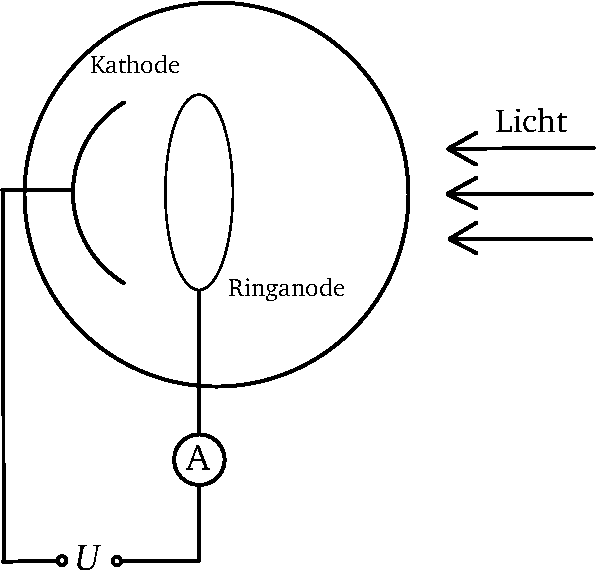
\includegraphics{../Zeichnungen/Photozelle.pdf}
    \caption{%
        Aufbau einer Photozelle mit Amperemeter und Gegenspannung $U$
    }
    \label{fig:Photozelle}
\end{figure}

In einem evakuiertem Behälter befinden sich eine Kathode und eine Ringanode,
zwischen denen eine Spannung anliegt. Die Anordnung wird mit Licht bestrahlt,
wodurch aus der Kathode Elektronen ausgelöst werden.

Liegt nun an der Kathode ein negatives und an der Anode ein positives Potenzial
an, werden die gelösten Elektronen in Richtung Anode beschleunigt. Mit dem
Amperemeter wird dann ein Strom gemessen.

Sind Kathode und Anode anders herum beschaltet, werden ausgelöste Elektronen in
Richtung Kathode beschleunigt, also abgebremst. Mit Hilfe der Spannung $U_0$,
bei der der Anodenstrom verschwindet, kann nun die kinetische Energie der
ausgelösten Elektronen bestimmt werden:
\[eU_0 = E_\text{kin}\]

Da die kinetische Energie die Differenz aus der Energie des Photons und der
Austrittsarbeit ist, gilt:
\[eU_0 = h\nu-W_\text{A}\]

Da man ein Auslösen von Elektronen aus der Anode verhindern möchte, wählt man
hier meist ein Material mit höherer Austrittsarbeit. Da so zwei Materialien mit
unterschiedlicher Austrittsarbeit verbunden sind, entsteht ein
Kontaktpotenzial, welches die Energiegleichung noch einmal verändert:
\begin{equation}
    U_0 = \frac he\nu - \frac{W_\text{A}}e - U_\text{K}
    \label{eq:Energiebilanz}
\end{equation}

Wenn man die Abhängigkeit der Gegenspannung $U_0$ von der Lichtfrequenz $\nu$
vermisst taucht das Konktaktpotenzial als Fehler bei der Bestimmung der
Austrittsarbeit (Achsenabschnitt) auf.

\section{Aufbau der Atomhülle}

\subsection{Linienbreite}

Die Spektrallinien werden mit einer gewissen Breite wahrgenommen. Dies hat
verschiedene Effekte, beginnend mit der natürlichen Linienbreite:

\begin{quote}
    Absolut scharfe Spektrallinien gibt es nicht. Selbst ein völlig isoliertes
    Atom könnte nur dann Licht einer absolut scharfen Frequenz aussenden, wenn
    es ununterbrochen Strahlen wüëde. Unabhängig vom speziellen Atommodell muss
    die emittierte Welle irgendwann aufhören. Jeder solche Abbruch verletzt
    aber die absolute Periodizität, und das Ergebnis ist nur noch als ein
    Kontinuum von Frequenzen darstellbar.
    \parencite[Abschnitt~14.3.2]{meschede-gerthsen_24}
\end{quote}

Die Verstimmung $\gamma$ ist der Kehrwert der Lebensdauer $\tau$ des Zustandes.
Für völlig isolierte Atome gilt $\gamma / \omega \approx \num{e-8}$.
\parencite[Abschnitt~14.3.2]{meschede-gerthsen_24}

Daraus folgt auch, dass die relative Verbreiterung der Wellenlängen diese Größe
hat:
\[
    \frac{\Deltaup \lambda}{\lambda}
    = \frac{\omega}{\Deltaup \omega}
    = \frac{\gamma}{\Deltaup \omega}
    \approx \num{e-8}
\]

Die Bewegung der Atome verursacht auch noch eine Dopplerverschiebung der
Frequenz, also auch der Wellenlänge. Diese Stärke dieser Verbreiterung ist
gegeben durch: \parencite{chemgapedia/spektrallinien/dopplerverbreiterung}
\[
    \Delta \nu_{1/2} = \num{7.16e-7} \cdot \nu_0
    \sqrt{\frac{T/\si\kelvin}{m/\si\atomicmassunit}}
\]

Interessant ist die relative Verbreiterung der Wellenlänge, daher teilen wir
durch $\nu_0$ erhalten
\begin{equation}
    \label{eq:dopplerverbreiterung}
    \frac{\Delta\lambda}\lambda = \num{7.16e-7} \cdot
    \sqrt{\frac{T/\si\kelvin}{m/\si\atomicmassunit}}
\end{equation}

\section{Spektroskopie}

\subsection{Gittergleichung}

Für die Bestimmung der Gitterkonstante im zweiten Versuchsteil wird eine
Gittergleichung benötigt, die nicht in der Anleitung gegeben ist. Diese muss
eine Gleichung sein, die die Abhängigkeit $(\omega_\text B, \omega_\text G,
\lambda) \mapsto g$ liefert.

Der Gangunterschied $\Delta$ bei einem Einfallswinkel $\alpha_0$ und einem
Austrittswinkel $\alpha_m$ für das Interferenzbild der Ordnung $m$ ist gegeben
durch: \parencite[Formel~368.16]{physik312-Anleitung}
\begin{equation}
    \label{eq:368.16}
    \Delta = g \cdot \del{\sin(\alpha_0) + \sin(-\alpha_m)} = m \lambda
\end{equation}

In diesem Versuch haben wir ein Reflexionsgitter, außerdem sind die Messwerte
$\omega_\text B$ und $\omega_\text G$. Die Umrechnung ist wie folgt:
\[
    \alpha_0 = \omega_\text G
    \eqnsep
    \alpha_m = \piup - \del{ \omega_\text B + \omega_\text G }
\]

Dies setzen wir in \eqref{eq:368.16} ein und erhalten:
\begin{equation}
    \label{eq:gittergleichung}
    g = \frac{m \lambda}{\sin(\omega_\text G) - \sin(\omega_\text B + \omega_\text G)}
\end{equation}

Dabei bestimmen wir noch den Fehler mit der Gaußschen Fehlerfortplanzung:
\[
    \Deltaup g
    = \frac{g^2}{m\lambda} \sqrt{
        \del{\del{\cos(\omegaG) - \cos(\omegaB +
        \omegaG)} \Deltaup \omegaG}^2
        +
        \del{\cos(\omegaB + \omegaG) \Deltaup \omegaB}^2
    }
\]

Sollte $\omega_\text B = \piup$ sein, darf es keinen Gangunterschied geben.
$\Delta$ wird 0. Die Vorzeichen sind also korrekt.

\subsection{CCD-Kamera}

Die CCD-Kamera misst die Intensität für verschiedene Pixel. Aus den Pixeln
berechnet sie den Winkel bei der Objektivbrennweite $f$ und Pixelnummer $p \in
[0, 2047]$ mit folgender Formel:
\[
    \beta = \arctan\del{\frac{(1024 - p) \cdot \SI{0.014}{\milli\meter}}f}
\]

Um nachher aus der Winkeldifferenz $\Deltaup \alpha$ auf eine
Wellenlängendifferenz schließen zu können, müssen wir \eqref{eq:lambda} nach
dem Bankwinkel $\omegaB$ ableiten:
\begin{equation}
    \label{eq:d_Lambda_d_beta}
    \dpd\lambda\omegaB = - g \cos(\omegaB + \omegaG)
\end{equation}

Mit diesem Ausdruck kann nun die Isotopieaufspaltung $\Deltaup \lambda$ (nicht
der Fehler von $\lambda$) berechnet werden mit:
\begin{equation}
    \label{eq:Delta_lambda}
    \Deltaup\lambda = \eval{\dpd\lambda\omegaB}_{\omegaB} \Deltaup\beta
\end{equation}

%%%%%%%%%%%%%%%%%%%%%%%%%%%%%%%%%%%%%%%%%%%%%%%%%%%%%%%%%%%%%%%%%%%%%%%%%%%%%%%
%                 Bestimmung des Planckschen Wirkungsquantums                 %
%%%%%%%%%%%%%%%%%%%%%%%%%%%%%%%%%%%%%%%%%%%%%%%%%%%%%%%%%%%%%%%%%%%%%%%%%%%%%%%

\FloatBarrier
\chapter{Bestimmung des Planckschen Wirkungsquantums}

\FloatBarrier
\section{Aufbau}

\begin{figure}[htbp]
    \centering
    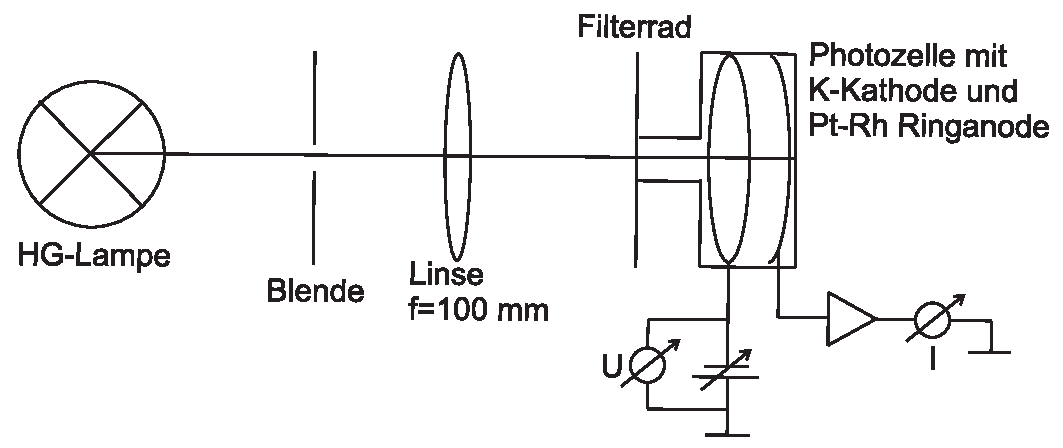
\includegraphics[width=\linewidth]{../Zeichnungen/P402-1.pdf}
    \caption{%
        \parencite[Abbildung~P402.1]{physik412-Anleitung}
    }
    \label{fig:P402.1}
\end{figure}

\FloatBarrier
\subsection{Justage}

Die Schutzkappe der Photozelle wird gelöst und das Filterrad auf $\lambda =
\SI{578}{\nano\meter}$ gestellt. Wenn die Hg-Dampflampe ihre volle Intensität
erreicht hat, können die Reflektionen auf Irisblende, Linse und
Interferenzfilter genutzt werden, um die Bauteile senkrecht und auf gleiche
Höhe auszurichten. Nun wird die Irisblende am Filterrad vollständig geöffnet
und die an der Lampe soweit geschlossen, dass der Lichtfleck auf der
Photokathode \SIrange{5}{10}{\milli\meter} Durchmesser hat. Dabei soll die
Ringanode nicht beleuchtet werden. Die Linse wird so verschoben, dass der
Lichfleck scharf abgebildet wird.

Im Anschluss wird die Schutzkappe so über die Photozelle gestülpt, dass
die Öffnung im Strahlengang liegt und die Irisblenden werden so weit
geschlossen, dass die Öffnung der Schutzkappe nicht überstrahlt wird.
Zuletzt wird, ohne dass die Justierung verändert wird, das Streulicht
begrenzende Rohr zwischen Schutzkappe und Filterrad angebracht.

\FloatBarrier
\subsection{Anschlüsse}

Der Anodenanschluss der Photozelle wird am negativen, der Kathodenanschluss am
positiven Ausgang eines Spannungsteilers angeschlossen, letzterer wird auf
Masse gezogen. Zwischen den Ausgängen wird ein Spannungsmesser angebracht. Der
Spannungsteiler liegt an einem regelbaren Netzgerät mit maximal \SI{12}{\volt}.

\FloatBarrier
\section{Durchführung}

Der Interferenzfilter wird auf das kurzwelligste Licht gestellt und die
Gegenspannung solange variiert, bis der Photostrom verschwindet. Nun wird der
Spannungsteiler so eingestellt, dass von da an die Maximalspannung etwa gleich
der gerade ermittelten Spannung ist. Für uns war das Verhältnis
$\frac{100}{550}$. Diese Einstellung wird für alle Messungen
beibehalten.

Nun wird zunächst der kleinste erreichbare Strom eingestellt. Dies ist $I_0$.
Die so eingestellte Gegenspannung ist ein erster Schätzwert für $U_0$.

Für die Kennlinie nimmt man Messpunkte von $U = \SI0{\volt}$ in
\SI{0.1}{\volt}-Abständen auf, bis $I = \SI0{\ampere}$ erreicht wird und geht
dann wieder mit gleichen Abständen zurück bis $U = \SI{0}{\volt}$.

Die Messungen für $I_0$, $U_0$ und die Kennlinie wird für alle Wellenlängen des
Filterrades durchgeführt.

Zuletzt wird mit veränderter Lichtintensität, bei deutlicher Vergrößerung bzw.
deutlicher Verringerung des Photostroms die Kennlinie der Wellenlänge $\lambda
= \SI{365}{\nano\meter}$ aufgenommem.

Unsere Messwerte befinden sich in Tabelle~\ref{tab:messwerte_365} bis
\ref{tab:messwerte_365_hoch}. In Abbildung~\ref{fig:Plot_365} bis
\ref{fig:Plot_365_hoch} sind diese graphisch dargestellt.

\begin{table}[htbp]
    \centering
    \begin{tabular}{SS|S}
        {$U_G / \si{\volt}$} &
        {$U / \si{\volt}$} &
        {$I / \si{\pico\ampere}$} \\
        \midrule
        %< for U_G, U, I in messwerte_365: ->%
        << U_G >> & << U >>  & << I >> \\
        %< endfor ->%
    \end{tabular}
    \caption{%
        Messwerte und mit der Verstärkung errechneter Photostrom zur Bestimmung
        von $U_0$. Wellenlänge \SI{365}{\nano\meter}.
    }
    \label{tab:messwerte_365}
\end{table}

\begin{table}[htbp]
    \centering
    \begin{tabular}{SS|S}
        {$U_G / \si{\volt}$} &
        {$U / \si{\volt}$} &
        {$I / \si{\pico\ampere}$} \\
        \midrule
        %< for U_G, U, I in messwerte_405: ->%
        << U_G >> & << U >>  & << I >> \\
        %< endfor ->%
    \end{tabular}
    \caption{%
        Messwerte und mit der Verstärkung errechneter Photostrom zur Bestimmung
        von $U_0$. Wellenlänge \SI{405}{\nano\meter}.
    }
    \label{tab:messwerte_405}
\end{table}

\begin{table}[htbp]
    \centering
    \begin{tabular}{SS|S}
        {$U_G / \si{\volt}$} &
        {$U / \si{\volt}$} &
        {$I / \si{\pico\ampere}$} \\
        \midrule
        %< for U_G, U, I in messwerte_436: ->%
        << U_G >> & << U >>  & << I >> \\
        %< endfor ->%
    \end{tabular}
    \caption{%
        Messwerte und mit der Verstärkung errechneter Photostrom zur Bestimmung
        von $U_0$. Wellenlänge \SI{436}{\nano\meter}.
    }
    \label{tab:messwerte_436}
\end{table}

\begin{table}[htbp]
    \centering
    \begin{tabular}{SS|S}
        {$U_G / \si{\volt}$} &
        {$U / \si{\volt}$} &
        {$I / \si{\pico\ampere}$} \\
        \midrule
        %< for U_G, U, I in messwerte_546: ->%
        << U_G >> & << U >>  & << I >> \\
        %< endfor ->%
    \end{tabular}
    \caption{%
        Messwerte und mit der Verstärkung errechneter Photostrom zur Bestimmung
        von $U_0$. Wellenlänge \SI{546}{\nano\meter}.
    }
    \label{tab:messwerte_546}
\end{table}

\begin{table}[htbp]
    \centering
    \begin{tabular}{SS|S}
        {$U_G / \si{\volt}$} &
        {$U / \si{\volt}$} &
        {$I / \si{\pico\ampere}$} \\
        \midrule
        %< for U_G, U, I in messwerte_578: ->%
        << U_G >> & << U >>  & << I >> \\
        %< endfor ->%
    \end{tabular}
    \caption{%
        Messwerte und mit der Verstärkung errechneter Photostrom zur Bestimmung
        von $U_0$. Wellenlänge \SI{578}{\nano\meter}.
    }
    \label{tab:messwerte_578}
\end{table}

\begin{table}[htbp]
    \centering
    \begin{tabular}{SS|S}
        {$U_G / \si{\volt}$} &
        {$U / \si{\volt}$} &
        {$I / \si{\pico\ampere}$} \\
        \midrule
        %< for U_G, U, I in messwerte_365_hoch: ->%
        << U_G >> & << U >>  & << I >> \\
        %< endfor ->%
    \end{tabular}
    \caption{%
        Messwerte und mit der Verstärkung errechneter Photostrom, bei höherer
        Intensität. Wellenlänge \SI{365}{\nano\meter}.
    }
    \label{tab:messwerte_365_hoch}
\end{table}

\begin{figure}
    \centering
    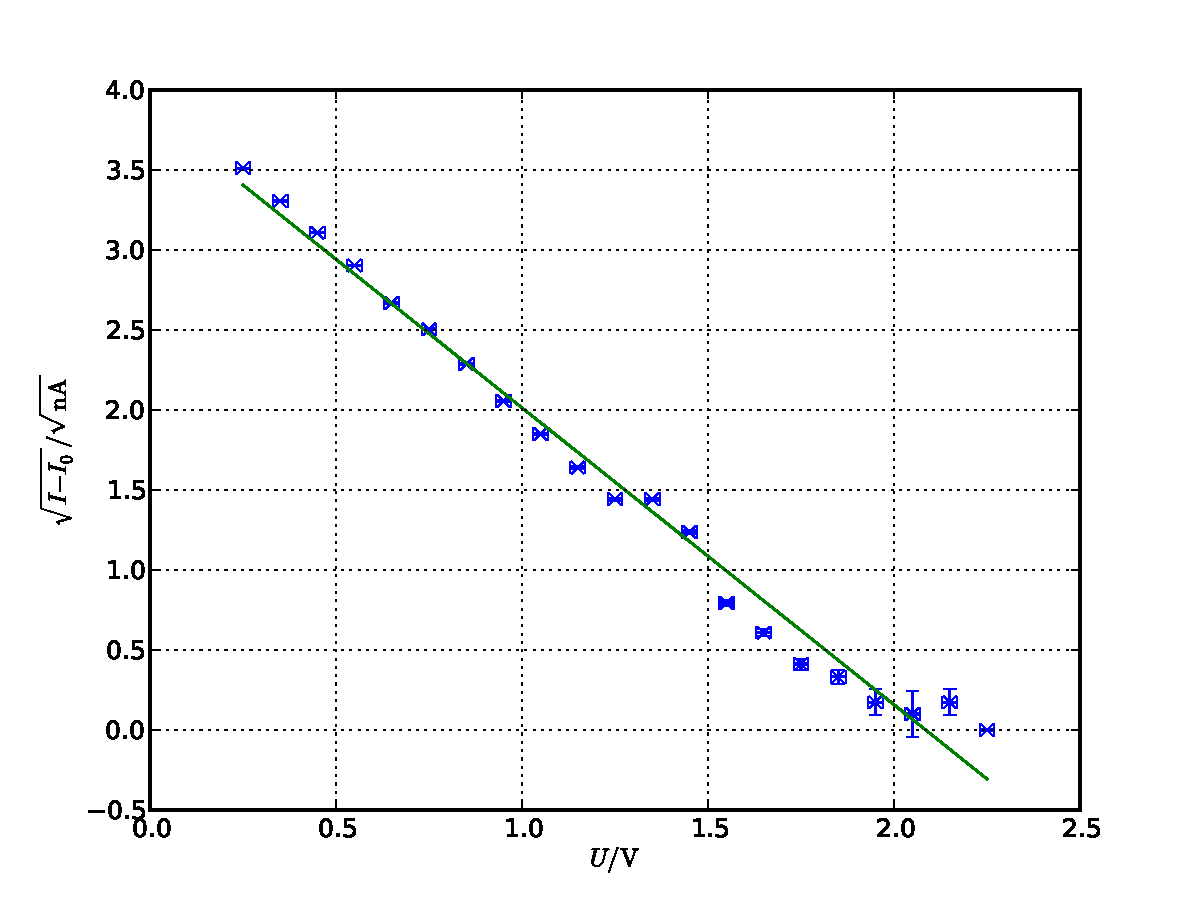
\includegraphics[width=\textwidth]{Plot-365.pdf}
    \caption{%
        Schaubild zur Messung bei $\lambda = \SI{365}{\nano\meter}$,
        einschließlich Anpassungsgerade nach der Least-Squares-Methode
    }
    \label{fig:Plot_365}
\end{figure}

\begin{figure}
    \centering
    \includegraphics[width=\textwidth]{Plot-405.pdf}
    \caption{%
        Schaubild zur Messung bei $\lambda = \SI{405}{\nano\meter}$,
        einschließlich Anpassungsgerade nach der Least-Squares-Methode
    }
    \label{fig:Plot_405}
\end{figure}

\begin{figure}
    \centering
    \includegraphics[width=\textwidth]{Plot-436.pdf}
    \caption{%
        Schaubild zur Messung bei $\lambda = \SI{436}{\nano\meter}$,
        einschließlich Anpassungsgerade nach der Least-Squares-Methode
    }
    \label{fig:Plot_436}
\end{figure}

\begin{figure}
    \centering
    \includegraphics[width=\textwidth]{Plot-546.pdf}
    \caption{%
        Schaubild zur Messung bei $\lambda = \SI{546}{\nano\meter}$,
        einschließlich Anpassungsgerade nach der Least-Squares-Methode
    }
    \label{fig:Plot_546}
\end{figure}

\begin{figure}
    \centering
    \includegraphics[width=\textwidth]{Plot-578.pdf}
    \caption{%
        Schaubild zur Messung bei $\lambda = \SI{578}{\nano\meter}$,
        einschließlich Anpassungsgerade nach der Least-Squares-Methode
    }
    \label{fig:Plot_578}
\end{figure}

\begin{figure}
    \centering
    \includegraphics[width=\textwidth]{Plot-365_hoch.pdf}
    \caption{%
        Schaubild zur Messung bei $\lambda = \SI{365}{\nano\meter}$ mit höherer
        Intensität. Es fällt auf, dass auch für höhere Gegenspannung der
        Sättigungsstrom beibehalten wird. Der Strom erreicht aber etwa bei
        der gleichen Gegenspannung $\SI{0}{\ampere}$
    }
    \label{fig:Plot_365_hoch}
\end{figure}

\FloatBarrier
\section{Auswertung}

Um $h$ zu bestimmen, ermitteln wir zunächst $U_0$ für die verschiedenen
Wellenlängen. Dazu suchen wir die Nullstelle unserer Anpassungsfunktion. Die
gefundenen Werte sind in Tabelle~\ref{tab:U_0} zu sehen.

\begin{table}[htbp]
    \centering
    \begin{tabular}{S|S|S}
        {$\lambda / \si{\nano\meter}$} &
        {$\nu / \si{\tera\hertz}$} &
        {$U_0 / \si{\volt}$} \\
        \midrule
        %< for wavelength, nu, U_0 in Tabelle_U_0 ->%
        << wavelength >> & << nu >>  & << U_0 >> \\
        %< endfor ->%
    \end{tabular}
    \caption{%
        Ermittelte Werte für $U_0$ mit zugehöriger Wellenlänge und Frequenz
    }
    \label{tab:U_0}
\end{table}

In Abbildung~\ref{fig:Plot_nu} ist $U_0$ gegen $\nu$, einschließlich
Anpassungsgerade gezeigt. Die Steigung der Geraden ist $\frac{h}{e}$, der
Achsenabschnitt ist $\frac{W_A}{e}+U_K$.

\begin{figure}
    \centering
    \includegraphics[width=\textwidth]{Plot_nu.pdf}
    \caption{%
        $U_0$ gegen $\nu$ einschließlich Anpassungsgerade. Aus der Steigung
        erhält man das Planck'sche Wirkungsquantum.
    }
    \label{fig:Plot_nu}
\end{figure}

Aus der Steigung der Anpassungsgeraden erhalten wir
\[
    h = \SI{<< h_photo >>}{\joule\second}
\]

Aus dem Achsenabschnitt erhalten wir
\[
    W_A \approx \SI{<< W_A >>}{\joule}
\]


%%%%%%%%%%%%%%%%%%%%%%%%%%%%%%%%%%%%%%%%%%%%%%%%%%%%%%%%%%%%%%%%%%%%%%%%%%%%%%%
%                                Balmer-Serie                                 %
%%%%%%%%%%%%%%%%%%%%%%%%%%%%%%%%%%%%%%%%%%%%%%%%%%%%%%%%%%%%%%%%%%%%%%%%%%%%%%%

\FloatBarrier
\chapter{Balmer-Serie}

In diesem Versuchsteil untersuchen wir die Balmer-Serie einer
Wasserstoff-Deuterium-Lampe mit einem Reflexionsgitter.

\FloatBarrier
\section{Aufbau}

Auf einer optischen Bank mit zwei Armen, deren gegenseitige Lage mit einer
Winkelskala bestimmt werden kann, werden die Komponenten aufgebaut. Dabei wird
auf dem ersten Arm die Lampe, eine Linse mit $f = \SI{50}{\milli\meter}$, ein
einstellbarer Spalt sowie ein Objektiv mit $f = \SI{150}{\milli\meter}$
aufgebaut.

In die Mitte wird das holographische Reflexionsgitter angebracht.

Auf dem zweiten Arm wird von der Mitte aus eine Linse mit $f =
\SI{300}{\milli\meter}$ und ein Okular mit Strichskala angebracht. Im weiteren
Verlauf dieses Teilversuchs wird noch eine CCD-Kamera angebracht.

\FloatBarrier
\subsection{Justierung}

Zuerst müssen wir den Aufbau justieren. Dazu benutzen wir die helle
Quecksilberlampe. Diese wird an das Ende des einen Arms gesetzt. Mit der ersten
Linse bilden wir die Lampe auf den Spalt ab. Der Spalt ist so angebracht, dass
die schrägen Flanken zur Lichtquelle ausgerichtet sind, und dass der Spalt
senkrecht ist.

Wir setzen das Objektiv zwischen Spalt und Gitter ein und drehen das Gitter so,
dass die Reflexion des Gitters wieder durch das Objektiv fällt und auf den
Spalt trifft. Der Abstand von Objektiv und Spalt ist grob dessen Brennweite $f
= \SI{150}{\milli\meter}$. Mit Hilfe dieser Autokollimationsanordnung stellen
wir die Position des Objektivs so ein, dass das Bild des Spaltes scharf ist.
Dadurch ist der Strahlengang nach dem Objektiv auf unendlich fokussiert.

Nun ist das Bild scharf eingestellt, liegt aber noch ein wenig neben dem Spalt.
Daher drehen wir jetzt das Gitter mit den Rändelschrauben so, dass das Bild
exakt in den Spalt fällt.

Die optische Bank klappen wir nun so zu, dass der Winkel $\omega_\text B$ im
Bereich von \SIrange{130}{170}{\degree} liegt. Wir lesen \SI{<< omega_B
>>}{\degree} ab.

Das Okular wird ans Ende des anderen Armes gestellt und so justiert, dass einer
von uns die Skala gut ablesen kann. Zuletzt setzen wir die Linse mit $f =
\SI{300}{\milli\meter}$ ein, damit wir im zweiten Arm die Spektrallinien durch
ein Teleskop beobachten können.

\FloatBarrier
\section{Durchführung}

\FloatBarrier
\subsection{Bestimmung der Gitterkonstanten}
\label{sec:gitterkonstante/durchführung}

Wir bestimmen die Gitterkonstante des Gitters durch eine Messung mit einer
Quecksilberdampflampe. Dazu lösen wir die Rändelschraube der Gittersäule und
drehen so lange, bis die erste Linie sichtbar wird. Um die Linie einfacher
erkennen zu können, weiten wir den Spalt auf und stellen ihn anschließend auf
\SI{0.1}{\milli\meter} zurück.

Mit der Objektivlinse des Beobachtungsteleskops können wir die Linien
scharfstellen, wir justieren so lange, bis diese es sind. Dann lesen wir den
Winkel des Gitters
$\omega_\text G$ ab. Die gemessenen Winkel sind in
Tabelle~\ref{tab:messdaten:gitterkonstante}. Anhand des Spektrums der Lampe
nehmen wir Wellenlängen an, siehe Tabelle.

\begin{table}[htbp]
    \centering
    \begin{tabular}{lSS|S}
        Farbe &
        {Winkel $\omega_\text G / \si\degree$} &
        {rel. Int.} &
        {Wellenlänge $\lambda / \si{\nano\meter}$} \\
        \midrule
        %< for farbe, omega_G, rel_int, lambda in messdaten_gitterkonstante: ->%
        << farbe >> & << omega_G >> +- << omega_G_err>> & << rel_int >> & <<
        lambda >> \\
        %< endfor ->%
    \end{tabular}
    \caption{%
        Messdaten für die Bestimmung der Gitterkonstanten mit der
        Quecksilberlampe. Hinter der senkrechten Linie sind die Wellenlängen,
        die wir anhand der Tabelle aus Anhang~\ref{sec:spektrum} annehmen.
    }
    \label{tab:messdaten:gitterkonstante}
\end{table}

\FloatBarrier
\subsection{Untersuchung der Balmer-Linien mit einem Okular}

Jetzt wiederholen wir diese Messung, jedoch mit der Balmer-Lampe. Dazu
entfernen wir die Quecksilberlampe und setzen die Wasserstofflampe ein. Mit der
ersten Linie bilden wir wieder die Lampe auf den Spalt ab. Dann führen die
gleiche Autokollimation wie im vorherigen Teil durch.

Die Rändelschraube an der Gittersäule wird gelöst und so weit gedreht, bis die
rote $\mathrm H_\alpha$-Linie zu sehen ist. Mit der Objektivlinse bilden wir
die Linie scharf ab.

Anschließend lesen wir den Gitterwinkel ab, den Bankwinkel haben wir
unverändert gelassen. Wir wiederholen dies für alle anderen Linien. Unsere
Messdaten sind in Tabelle~\ref{tab:messdaten:balmer-okular}.

\begin{small}
    Der Anleitung nach hätten wir hier die Aufspaltung $d$ der Linien
    mit der Skala im Okular abschätzen sollen. Dies haben wir leider versäumt.
\end{small}

\begin{table}[htbp]
    \centering
    \begin{tabular}{lSS}
        Farbe &
        {$\omega_\text G / \si\degree$} &
        {rel. Int.} \\
        \midrule
        %< for farbe, omega_G, rel_int in messdaten_balmer: ->%
        << farbe >> & << omega_G >> +- << omega_G_err>> & << rel_int >> \\
        %< endfor ->%
    \end{tabular}
    \caption{%
        Messdaten für die Balmer-Lampe, bestimmt mit einem Okular
    }
    \label{tab:messdaten:balmer-okular}
\end{table}

\FloatBarrier
\subsection{Untersuchung der Balmer-Linien mit einer CCD-Kamera}

Jetzt wird das Okular durch eine CCD-Kamera ersetzt. Wir starten das Programm
„VideoCom“ und stellen im Menü „Kalibrierung / Theorievergleich“
(\keystroke{F5}) im Register „Beugungswinkel“ die Brennweite $f =
\SI{300}{\milli\meter}$ der Objektivlinse ein. Die Belichtungszeit stellen wir
auf Stufe 8. Wir aktivieren die Messung mit \keystroke{F9}.

Die roten Balmer-Linien müssen auf die Mitte der CCD-Zeile abgebildet werden,
daher drehen wir das Gitter entsprechend. Mit der Objektivlinse stellen wir die
Linien scharf, das Ergebnis kontrollieren wir auf dem Monitor.

Mit der Schaltfläche „$\sum_1$“ starten wir die Mittelwertsbildung. Sobald wir
mit dem Ergebnis zufrieden sind, stoppen wir die Messung mit \keystroke{F9}.
Die Messdatentabelle speichern wir mit „Tabelle Kopieren“ in einer Textdatei.

Diesen Vorgang wiederholen wir für alle Linien. Unsere Messdaten sind in
im Anhang~\ref{sec:pc_messwerte}.

\FloatBarrier
\section{Auswertung}

\FloatBarrier
\subsection{Bestimmung der Gitterkonstanten}

Mithilfe der Gittergleichung \eqref{eq:gittergleichung} können wir die
Gitterkonstante bestimmen.

Die errechneten Werte sind in Tabelle~\ref{tab:gitterkonstante}. Die gleichen
Daten haben wir in Abbildung~\ref{fig:gitterkonstanten} dargestellt, um einfach
erkennen zu können, ob einzelne Wellenlängen falsch abgeschätzt worden sind.

\begin{table}[htbp]
    \centering
    \begin{tabular}{SS|S}
        {$\omegaG / \si{\radian}$} &
        {$\lambda / \si{\nano\meter}$} &
        {$g / \si{\nano\meter}$} \\
        \midrule
        %< for omega_G_val, lambda, g in tabelle_gitterkonstante: ->%
        << omega_G_val >> & << lambda >>  & << g >> \\
        %< endfor ->%
    \end{tabular}
    \caption{%
        Berechnete Gitterkonstanten aus den Messwerten aus
        Abschnitt~\ref{sec:gitterkonstante/durchführung},
        Tabelle~\ref{tab:messdaten:gitterkonstante}.
    }
    \label{tab:gitterkonstante}
\end{table}

\begin{figure}[htbp]
    \centering
    \includegraphics[width=\linewidth]{g.pdf}
    \caption{%
        Berechnete Gitterkonstanten für die einzelnen Wellenlängen. Bei einer
        idealen Messung sollte eine horizontale Gerade bei einem festen Wert
        für $g$ herauskommen. Abweichungen nach oben oder unten bedeuten, dass
        die Wellenlänge über- oder unterschätzt worden ist. Die Wellenlängen im
        blauen Bereich konnten wir anscheinend relativ gut zuordnen. Die beiden
        roten Wellenlängen sind im Vergleich viel zu groß. Jedoch gibt es keine
        kleineren Wellenlängen im angegeben Spektrum, die wir benutzen könnten.
        Die beiden roten Wellenlängen im Spektrum haben wir den beiden
        Messungen zugeordnet.
    }
    \label{fig:gitterkonstanten}
\end{figure}

Wir kombinieren die verschiedenen Werte von $g$ mit einem gewichteten
arithmetischen Mittel, wobei wir als Gewicht $1/\Deltaup g$
verwenden.\footnote{Ein einfacher Mittelwert hätte $g = \SI{<< g_mean
>>}{\meter}$ ergeben.} Die Fehler kombinieren wir quadratisch mit dem gleichen
Mittelwert und teilen noch durch $\sqrt n$.
\[
    g = \SI{<< g_average >>}{\meter}
\]

\FloatBarrier
\subsection{Bestimmung der Balmerlinien mit Okular}

Jetzt haben wir die Gitterkonstante und können die Gittergleichung zur
Wellenlängenbestimmung nutzen. Da wir nur die erste Ordnung benutzt haben, ist
$m = 1$.
\begin{equation}
    \label{eq:lambda}
    \lambda =
    \abs{g \cdot \del{\sin(\omega_\text G) - \sin(\omega_\text B + \omega_\text
    G)}}
\end{equation}

Hier berechnet sich der Fehler wie folgt:
\[
    \Deltaup \lambda
    =
    \sqrt{
        \del{\frac{\lambda}g \Deltaup g}^2
        +
        \del{g \del{\cos(\omegaG) - \cos(\omegaB + \omegaG)} \Deltaup
        \omegaG}^2
        +
        \del{g \cos(\omegaB + \omegaG) \Deltaup \omegaB}^2
    }
\]

\begin{table}[htbp]
    \centering
    \begin{tabular}{lSS|S}
        Farbe &
        {$\omega_\text G / \si{\milli\radian}$} &
        {rel. Int.} &
        {$\lambda / \si{\nano\meter}$} \\
        \midrule
        %< for farbe, omega_G, rel_int, lambda_ in tabelle_balmer: ->%
        << farbe >> & << omega_G >> & << rel_int >> & <<
        lambda_ >> \\
        %< endfor ->%
    \end{tabular}
    \caption{%
        Wellenlängen zu den Balmerlinien.
    }
    \label{tab:balmer-okular}
\end{table}

Die zu erwartenden Wellenlängen berechnen sich nach:
\[
    \lambda = \frac{c h}{E_\text{Ryd}} \del{\frac 14 - \frac 1{n^2}}^{-1}
\]

Die davon sichtbaren sind: \SIlist{<< balmer_berechnet_nm >>}{\nano\meter}.

\subsubsection{Bestimmung der Ballmerlinien mit CCD-Zeile}

Die Daten, die wir mit dem PC aufgenommen haben, stellen wir graphisch dar.

An einen ausgewählten Bereich (im Plot markiert) passen wir eine Gaußfunktion
an:
\[
    I(\alpha) = a \exp\del{- \frac{(\alpha - \alpha_0)^2}{2 \sigma}}
\]

Die Halbwertsbreite $H$ ist gegeben als: \parencite{wikipedia/gaussian_function}
\[
    H = 2 \sqrt{2 \ln(2)} \sigma
\]

\subsubsection{Erste rote Linie}

Die erste rote Linie (Abbildung~\ref{fig:rot}) konnten wir gut abbilden und die
Isotopieaufspaltung beobachten.

Wir benutzen im Graph die Datenpunkte \numrange{<< rot_lower >>}{<< rot_upper
>>}. Für das Hauptmaximum beziehen wir aus der Menge der gezeigten Punkte die
Punkte \numrange{<< rot_primary_lower >>}{<< rot_primary_upper >>} ein. Für das
Nebenmaximum die Punkte \numrange{<< rot_secondary_lower >>}{<<
rot_secondary_upper >>}. Negative Indizes zählen vom Ende aus.

Es wurde ein konstantes Untergrundsignal von \num{<< rot_underground >>}
abgezogen. An die markierten Datenpunkte wurde jeweils eine Gaußfunktion
angepasst. 

Für das Hauptmaximum erhalten wir einen Winkel
von \SI{<< rot_primary_center >>}{\degree} und eine Halbwertsbreite von
\SI{<< rot_primary_fwhm >>}{\degree}. Das Nebenmaximum liegt bei \SI{<<
rot_secondary_center >>}{\degree} und hat eine Halbwertsbreite von \SI{<<
rot_secondary_fwhm >>}{\degree}.

Daraus erhalten wir eine Winkeldifferenz von \SI{<< rot_differenz >>}{\degree}.
Nach \eqref{eq:d_Lambda_d_beta} ist dies eine Wellenlängendifferenz von
$\Deltaup \lambda = \SI{<<
rot_Delta_lambda >>}{\meter}$. Das $\omegaG$, das wir dort eingesetzt haben,
hatten wir bei der Messung mit der CCD-Zeile nicht notiert. Jedoch haben wir
den Bankwinkel nicht verändert, so dass wir hier für den Gitterwinkel den Wert
von $\omegaG = \SI{<< rot_omega_G >>}{\degree}$ benutzen, den wir vorher für
die hellste rote Linie erhalten haben.

Die relative Aufspaltung ist:
\[
    \frac{\Deltaup \lambda}{\lambda}
    = \frac{\SI{<< rot_Delta_lambda >>}\meter}{\SI{<< rot_lambda >>}\meter}
    =  \num{<< rot_rel_aufspaltung >>}
\]

\begin{figure}[htbp]
    \centering
    \includegraphics[width=\linewidth]{rot.pdf}
    \caption{%
        Graph der Daten zur ersten roten Linie. Gezeigt werden nur die
        Datenpunkte \num{<< rot_lower >>} bis \num{<< rot_upper >>}
        (Arrayindex). Es wurde ein Untergrundsignal von \num{<< rot_underground
        >>} abgezogen. An die Punkte \numrange{<< rot_primary_lower >>}{<<
        rot_primary_upper >>} aus der gezeigten Punktmenge wurde eine
        Gaußfunktion angepasst. Der Mittelwert dieses Hauptmaximums liegt bei
        \SI{<< rot_primary_center >>}{\degree} und hat eine Halbwertsbreite von
        \SI{<< rot_primary_fwhm >>}{\degree}. An die Punkte \numrange{<<
        rot_secondary_lower >>}{<< rot_secondary_upper >>} wurde die gleiche
        Funktion angepasst. Dieses Nebenmaximum liegt bei \SI{<<
        rot_secondary_center >>}{\degree} und hat eine Halbwertsbreite von
        \SI{<< rot_secondary_fwhm >>}{\degree}.
    }
    \label{fig:rot}
\end{figure}

\subsubsection{Zweite rote Linie}

Hier gehen wir analog vor, siehe Abbildung~\ref{fig:rot2}. Da wir hier keine
Aufspaltung erkennen konnten, entfällt die Anpassung einer weiteren Gaußkurve
und die Bestimmung der Aufspaltung.

\begin{figure}[htbp]
    \centering
    \includegraphics[width=\linewidth]{rot2.pdf}
    \caption{%
        Graph der Daten zur zweiten roten Linie. Gezeigt werden nur die
        Datenpunkte \num{<< rot2_lower >>} bis \num{<< rot2_upper >>}
        (Arrayindex). Es wurde ein Untergrundsignal von \num{<< rot2_underground
        >>} abgezogen. An die Punkte \numrange{<< rot2_primary_lower >>}{<<
        rot2_primary_upper >>} aus der gezeigten Punktmenge wurde eine
        Gaußfunktion angepasst. Der Mittelwert dieses Hauptmaximums liegt bei
        \SI{<< rot2_primary_center >>}{\degree} und hat eine Halbwertsbreite von
        \SI{<< rot2_primary_fwhm >>}{\degree}.
    }
    \label{fig:rot2}
\end{figure}

\subsubsection{Grüne Linie}

In Abbildung~\ref{fig:gruen} ist die grüne Linie zu erkennen, wieder ohne
Aufspaltung.

\begin{figure}[htbp]
    \centering
    \includegraphics[width=\linewidth]{gruen.pdf}
    \caption{%
        Graph der Daten zur grünen Linie. Gezeigt werden nur die Datenpunkte
        \num{<< gruen_lower >>} bis \num{<< gruen_upper >>} (Arrayindex). Es
        wurde ein Untergrundsignal von \num{<< gruen_underground >>} abgezogen.  An die
        Punkte \numrange{<< gruen_primary_lower >>}{<< gruen_primary_upper >>} aus
        der gezeigten Punktmenge wurde eine Gaußfunktion angepasst. Der
        Mittelwert dieses Hauptmaximums liegt bei \SI{<< gruen_primary_center
        >>}{\degree} und hat eine Halbwertsbreite von \SI{<< gruen_primary_fwhm
        >>}{\degree}.
    }
    \label{fig:gruen}
\end{figure}

\subsubsection{Erste cyane Linie}

In Abbildung~\ref{fig:cyan} ist die erste cyane Linie, auch wieder ohne
Aufspaltung.

\begin{figure}[htbp]
    \centering
    \includegraphics[width=\linewidth]{cyan.pdf}
    \caption{%
        Graph der Daten zur ersten cyanen Linie. Gezeigt werden nur die
        Datenpunkte \num{<< cyan_lower >>} bis \num{<< cyan_upper >>}
        (Arrayindex). Es wurde ein Untergrundsignal von \num{<< cyan_underground
        >>} abgezogen. An die Punkte \numrange{<< cyan_primary_lower >>}{<<
        cyan_primary_upper >>} aus der gezeigten Punktmenge wurde eine
        Gaußfunktion angepasst. Der Mittelwert dieses Hauptmaximums liegt bei
        \SI{<< cyan_primary_center >>}{\degree} und hat eine Halbwertsbreite von
        \SI{<< cyan_primary_fwhm >>}{\degree}.
    }
    \label{fig:cyan}
\end{figure}

\subsubsection{Zweite cyane Linie}

In Abbildung~\ref{fig:cyan2} ist die zweite cyane Linie, auch wieder ohne
Aufspaltung.

\begin{figure}[htbp]
    \centering
    \includegraphics[width=\linewidth]{cyan2.pdf}
    \caption{%
        Graph der Daten zur zweiten cyanen Linie. Gezeigt werden nur die
        Datenpunkte \num{<< cyan2_lower >>} bis \num{<< cyan2_upper >>}
        (Arrayindex). Es wurde ein Untergrundsignal von \num{<< cyan2_underground
        >>} abgezogen. An die Punkte \numrange{<< cyan2_primary_lower >>}{<<
        cyan2_primary_upper >>} aus der gezeigten Punktmenge wurde eine
        Gaußfunktion angepasst. Der Mittelwert dieses Hauptmaximums liegt bei
        \SI{<< cyan2_primary_center >>}{\degree} und hat eine Halbwertsbreite von
        \SI{<< cyan2_primary_fwhm >>}{\degree}.
    }
    \label{fig:cyan2}
\end{figure}

\subsubsection{Blaue Linie}

In Abbildung~\ref{fig:blau} ist die blaue Linie. Hier ist eine Aufspaltung zu
erkennen. Wir passen wie bei der ersten roten Linie zwei Gaußfunktionen an.

Daraus erhalten wir eine Winkeldifferenz von \SI{<< blau_differenz >>}{\degree}.
Nach \eqref{eq:d_Lambda_d_beta} ist dies eine Wellenlängendifferenz von
$\Deltaup \lambda = \SI{<<
blau_Delta_lambda >>}{\meter}$. Das $\omegaG$, das wir dort eingesetzt haben,
hatten wir bei der Messung mit der CCD-Zeile nicht notiert. Jedoch haben wir
den Bankwinkel nicht verändert, so dass wir hier für den Gitterwinkel den Wert
von $\omegaG = \SI{<< blau_omega_G >>}{\degree}$ benutzen, den wir vorher für
die blaue Linie erhalten haben.

Die relative Aufspaltung ist:
\[
    \frac{\Deltaup \lambda}{\lambda}
    = \frac{\SI{<< blau_Delta_lambda >>}\meter}{\SI{<< blau_lambda >>}\meter}
    =  \num{<< blau_rel_aufspaltung >>}
\]

\begin{figure}[htbp]
    \centering
    \includegraphics[width=\linewidth]{blau.pdf}
    \caption{%
        Graph der Daten zur blauen Linie. Gezeigt werden nur die Datenpunkte
        \num{<< blau_lower >>} bis \num{<< blau_upper >>} (Arrayindex). Es
        wurde ein Untergrundsignal von \num{<< blau_underground >>} abgezogen.  An die
        Punkte \numrange{<< blau_primary_lower >>}{<< blau_primary_upper >>}
        aus der gezeigten Punktmenge wurde eine Gaußfunktion angepasst. Der
        Mittelwert dieses Hauptmaximums liegt bei \SI{<< blau_primary_center
        >>}{\degree} und hat eine Halbwertsbreite von \SI{<< blau_primary_fwhm
        >>}{\degree}. An die Punkte \numrange{<< blau_secondary_lower >>}{<<
        blau_secondary_upper >>} wurde die gleiche Funktion angepasst. Dieses
        Nebenmaximum liegt bei \SI{<< blau_secondary_center >>}{\degree} und
        hat eine Halbwertsbreite von \SI{<< blau_secondary_fwhm >>}{\degree}.
    }
    \label{fig:blau}
\end{figure}

\subsubsection{Linienbreiten}

In Tabelle~\ref{tab:linienbreiten} haben wir die Linienbreiten noch einmal
zusammengestellt. Mit der Formel, mit der wir auch die Isotopieaufspaltung
$\Deltaup \alpha$ in Grad in eine Wellenlängendifferenz $\Deltaup \lambda$
umgewandelt haben, wandeln wir die Breite in eine Wellenländendifferenz um.
Dabei benutzen wir als Bankwinkel $\omegaB$ den Winkel, den wir für diese Linie
mit dem Okular erhalten hatten.

\begin{table}[htbp]
    \centering
    \begin{tabular}{lSSS}
        Linie & {$\Deltaup\alpha / \si{\micro\degree}$} & {$\Deltaup\lambda /
    \si{\nano\meter}$} & {Aufspaltung / $10^{-3}$} \\
        \midrule
        %< for farbe, fwhm, linienbreite, gamma in zusammenfassung: >%
        << farbe >> & << fwhm >> & << linienbreite >> & << gamma >> \\
        %< endfor >%
    \end{tabular}
    \caption{%
        Zusammenstellung der Linienbreiten, die wir aus den Daten der CCD-Zeile
        bestimmt haben.
    }
    \label{tab:linienbreiten}
\end{table}

\subsection{Bestimmung der Rydbergkonstanten}

Die Rydbergkonstante ist definiert als: \parencite[Umschlag]{meschede-gerthsen_24}
\[
    R_\infty = \frac{\alpha^2 m_\text e c}{2 h}
\]

Zusammen mit der Feinstrukturkonstante $\alpha = e^2/(4\piup \varepsilon_0
\hbar c)$: \parencite[Umschlag]{meschede-gerthsen_24}
\[
    R_\infty = \frac{e^4 m_\text e}{8 \varepsilon_0^2 c h^3}
\]

Dies deckt sich mit \cite{wikipedia/Rydbergkonstante}.

Die Rydbergkonstante erhalten wir, in dem wir aus den Wellenlängen die
Energiedifferenzen der Übergänge errechnen und das passende Energieniveau
finden, von dem der Übergang gestartet ist.

Die von uns gemessenen Wellenlängen waren: \SIlist{<< balmer_lambda_nm >>}{\meter}.

Zu erwartende Wellenlängen sind für die Übergänge $n \to 2$: \SIlist{<<
balmer_berechnet_nm >>}{\nano\meter}.

Die ehesten Kandidaten sind:
\begin{itemize}
    \item $\SI{<< balmer_lambda[0] >>}\meter \approx \SI{<<
        balmer_berechnet[1] >>}\meter$, $5 \to 2$.

    \item $\SI{<< balmer_lambda[2] >>}\meter \approx \SI{<<
        balmer_berechnet[2] >>}\meter$, $4 \to 2$.

    \item $\SI{<< balmer_lambda[6] >>}\meter \approx \SI{<<
        balmer_berechnet[3] >>}\meter$, $3 \to 2$.
\end{itemize}

Diese drei Punkte stellen wir in Abbildung~\ref{fig:balmer_ausgesucht}
graphisch dar. An die Punkte passen wir folgende Funktion an:
\[
    \lambda(n) = C \del{\frac{1}{2^2} - \frac{1}{n^2}}^{-1}
\]

\begin{figure}[htbp]
    \centering
    \includegraphics[width=\linewidth]{balmer_ausgesucht.pdf}
    \caption{%
        Ausgesuchte Balmerlinien.
    }
    \label{fig:balmer_ausgesucht}
\end{figure}

Wobei
\[
    C = \frac{1}{R_\infty}
    = \frac{8 \varepsilon_0^2 c h^3}{e^4 m_\text e}
\]

Dies lösen wir nach dem gesuchten $h$ auf:
\[
    h = \del{\frac{e^4 m_\text e C}{8 \varepsilon_0^2 c}}^{1/3}
\]

Und erhalten für $h$:
\[
    h = \SI{<< h >>}{\joule\second}
\]

%%%%%%%%%%%%%%%%%%%%%%%%%%%%%%%%%%%%%%%%%%%%%%%%%%%%%%%%%%%%%%%%%%%%%%%%%%%%%%%
%                                 Diskussion                                  %
%%%%%%%%%%%%%%%%%%%%%%%%%%%%%%%%%%%%%%%%%%%%%%%%%%%%%%%%%%%%%%%%%%%%%%%%%%%%%%%

\FloatBarrier
\chapter{Diskussion}

\section{Messfehler im ersten Teil}

Im ersten Teil des Versuches konnten wir durch die Abschirmung das meiste
Streulicht heraushalten und somit wahrscheinlich relativ fehlerarm messen.
Steulicht würde jedoch dazu führen, dass alle Daten eine konstante Erhöhung
haben und die Nullstellen somit falsch herauskommen.

Durch die große Verstärkung könnte es sein, dass bereits kleine statische
Ladungen das Ergebnis kurzzeitig verfälscht haben. Jedoch sollte sich das im
Mittel ausgleichen.

Bei der Messung haben die Ausgangsspannung teilweise sehr stark geschwankt.
Dies haben wir beim Ablesen direkt im Messfehler festgehalten.

\section{Bestimmung der Nullstellen}

Wir haben die Nullstellen der Anpassungsgeraden numerisch bestimmen lassen. Für
die Anpassungsgerade haben wir zwar Parameter mit Fehlerangaben erhalten,
jedoch sind die Koordinaten miteinander korreliert, wodurch wir nicht sicher
sein können, ob der Fehler der Nullstelle bereits dadurch abgedeckt wird.
Eventuell verstärkt sich der Fehler bei unserem Verfahren deutlich stärker, als
wir das erwartet haben.

\section{Messfehler im zweiten Teil}

Bei der Bestimmung der Gitterkonstanten ist es nicht möglich, eine horizontale
Gerade durch die einzelnen Gitterkonstanten zu legen, so dass diese innerhalb
der Fehlerbereiche ist. Es ist schwer, den Fehler durch die Wahl der falschen
Wellenlänge im Spektrum zu quantifizieren, jedoch ist die Unsicherheit dort
größer als durch die Messung von $\omegaG$ allein.

Wir konnten die Aufspaltung im Okular nicht erkennen, mit der CCD-Zeile nur für
die helle rote Linie. Da das Auflösungsvermögen des Gitters eigentlich
ausreichen sollte, um die Aufspaltung auch bei anderen Spektrallinien sehen zu
können, muss etwas anderes die Auflösung begrenzt haben. Wahrscheinlich ist
viel Auflösungsvermögen bei der Justage der Linsen verloren gegangen, weil
diese nicht alle auf höhe der optischen Achse waren.

Der Literaturwert für $h$ liegt nicht mehr im Fehlerbereich des Wertes, den wir
im zweiten Teil mit der Balmer-Lampe erhalten haben. Hier haben wir
offensichtlich die Fehler unterschätzt.

\section{Weitere Spektrallinien}

Wasserstoff und Deuterium liegen in der Gasentladungslampe nicht als Atome vor,
da diese freien Radikale sich direkt zu Wasserstoffgas verbinden würden. Als
Molekül hätte es jedoch ein Spektrum mit Banden und Linien, nicht
ausschließlich Linien. Siehe zum Beispiel
\cite[Abbildung~14.15]{meschede-gerthsen_24}.

In einer solchen Wasserstofflampe ist Wasserdampf, in dem sich hin und wieder
ein Wasserstoffatom löst. Dadurch erscheint das Spektrum ohne Banden.
\parencite[Abschnitt~2.1]{leybold/balmer_lampe}
\parencite{wikipedia/gas_discharge_lamp}

Allerdings könnte der $\mathrm{\mathsf{HO}}$-Rumpf auch noch schwingen und eine
grüne Linie erzeugen.

\section{Linienbreite}

\subsection{Dopplerverbreiterung}

Nach \eqref{eq:dopplerverbreiterung} erhalten wir bei $T = \SI{1000}{\kelvin}$
und $m = \SI{1}{\atomicmassunit}$ eine Verbreiterung von \num{<< doppler >>}.

\subsection{Natürliche Linienbreite}

Die natürliche Linienbreite mit ihren \num{e-8} ist deutlich geringer als die
Dopplerverbreiterung und kann hier vernachlässigt werden.

\subsection{Vergleich mit aufgenommenen Linien}

Für die erste rote und die blaue Linie ist die Verbreiterung recht klein,
allerdings immer noch mehr als eine Größenordnung größer als die
Dopplerverbreiterung. Die anderen Linien sind deutlich breiter, dort wurde
anscheinend schlecht fokussiert.

Somit ist unsere Linienbreite durch die Abbildung in unserem Aufbau begrenzt.

\section{Auflösungsvermögen des Gitters}

Wir haben in erster Ordnung betrachtet und wahrscheinlich das ganze Gitter
ausgeleuchtet, also eine Breite von \SI{<< d >>}{\meter}.
Daher erhalten wir ein Auflösungsvermögen von:
\[
    \frac{\Deltaup \lambda}{\lambda} = \num{<< aufl >>}
\]

Dies würde für die Isotopieaufspaltung reichen, jedoch waren unsere
Linsensysteme nicht entsprechend genau.

\section{Isotopieaufspaltung}

Die Aufspaltung bei der blauen Linie ist sehr groß, gut einen Faktor zehn
größer als bei der ersten roten Linie. Daher gehen wir davon aus, dass das
Nebenmaximum nicht von der Aufspaltung stammt, sondern eine Linie eines anderen
Übergangs ist. Somit bleibt uns nur die Aufspaltung der roten Linie.

Dennis~P. sagte uns nach dem Versuch, dass in diesem Versuch auch nur die
Aufspaltung der roten Linie sinnvoll zu erkennen ist.

Zu erwarten ist laut \cite{PHManual/atomic} eine Aufspaltung in der
Größenordnung \SI{0.25}{\percent}, also \num{2.5e-4}. Beobachtet haben wir
jedoch \num{<< rot_rel_aufspaltung >>}, das zwei Größenordnungen größer ist.
Entweder haben wir falsch gerechnet, oder das Nebenmaximum hat mit der
Isotopieaufspaltung nichts zu tun.

%%%%%%%%%%%%%%%%%%%%%%%%%%%%%%%%%%%%%%%%%%%%%%%%%%%%%%%%%%%%%%%%%%%%%%%%%%%%%%%
%                               Zusammenfassung                               %
%%%%%%%%%%%%%%%%%%%%%%%%%%%%%%%%%%%%%%%%%%%%%%%%%%%%%%%%%%%%%%%%%%%%%%%%%%%%%%%

\FloatBarrier
\chapter{Zusammenfassung}

Wir haben das Planck'sche Wirkungsquantum durch zwei unabhängige Verfahren
bestimmt. Zuerst haben wir den Photoeffekt ausgenutzt, in dem die verschiedenen
Farben des Lichts verschiedene Energien pro Photon tragen. Im zweiten Teil
haben wir die Energieniveaus des Wasserstoffs benutzt, in denen auch das
Wirkungsquantum steckt.

Der Wert, den wir durch den Photoeffekt erhalten haben, ist:
\[
    h_\text{Photo} = \SI{<< h_photo >>}{\joule\second}
\]

Der Wert für das Wirkungsquantum, den wir über die Balmer-Linien erhalten
haben, ist:
\[
    h_\text{Balmer} = \SI{<< h >>}{\joule\second}
\]

Beide Werte liegen mehr als eine Standardabweichung vom Literaturwert
\SI{6.626e-34}{\joule\second} entfernt, damit sind die Fehler zu klein.

%%%%%%%%%%%%%%%%%%%%%%%%%%%%%%%%%%%%%%%%%%%%%%%%%%%%%%%%%%%%%%%%%%%%%%%%%%%%%%%
%                                   Anhang                                    %
%%%%%%%%%%%%%%%%%%%%%%%%%%%%%%%%%%%%%%%%%%%%%%%%%%%%%%%%%%%%%%%%%%%%%%%%%%%%%%%

\FloatBarrier
\begin{appendix}
    \chapter{PC Messwerte}
    \label{sec:pc_messwerte}

    Dies sind die von „VideoCom“ erzeugten Daten. Hier abgedruckt sind nur die
    Datenpunkte, die auch im Plot verwendet worden sind. Unter jeder Tabelle
    ist eine URL zur vollständigen Datei angegeben. In der ersten Spalte ist
    der Winkel $\alpha$ in $\si\degree$, in der zweiten Spalte die relative
    Intensität.

    \section{Erste rote Linie (rot.txt)}
    \begin{multicols}{5}
        \inputminted[tabsize=4, firstline=<< rot_lower >>, lastline=<< rot_upper >>, fontsize=\footnotesize]{text}{../Messwerte/rot.txt}
    \end{multicols}

    Die vollständige Datei gibt es hier: \\
    \url{https://raw.github.com/martin-ueding/physik412-Protokolle/master/402/Messwerte/rot.txt}

    \section{Zweite rote Linie (rot2.txt)}
    \begin{multicols}{5}
        \inputminted[tabsize=4, firstline=<< rot2_lower >>, lastline=<< rot2_upper >>, fontsize=\footnotesize]{text}{../Messwerte/rot2.txt}
    \end{multicols}

    Die vollständige Datei gibt es hier: \\
    \url{https://raw.github.com/martin-ueding/physik412-Protokolle/master/402/Messwerte/rot2.txt}

    \section{Grüne Linie (gruen.txt)}
    \begin{multicols}{5}
        \inputminted[tabsize=4, firstline=<< gruen_lower >>, lastline=<< gruen_upper >>, fontsize=\footnotesize]{text}{../Messwerte/gruen.txt}
    \end{multicols}

    Die vollständige Datei gibt es hier: \\
    \url{https://raw.github.com/martin-ueding/physik412-Protokolle/master/402/Messwerte/gruen.txt}

    \section{Erste cyane Linie (cyan.txt)}
    \begin{multicols}{5}
        \inputminted[tabsize=4, firstline=<< cyan_lower >>, lastline=<< cyan_upper >>, fontsize=\footnotesize]{text}{../Messwerte/cyan.txt}
    \end{multicols}

    Die vollständige Datei gibt es hier: \\
    \url{https://raw.github.com/martin-ueding/physik412-Protokolle/master/402/Messwerte/cyan.txt}

    \section{Zweite cyane Linie (cyan2.txt)}
    \begin{multicols}{5}
        \inputminted[tabsize=4, firstline=<< cyan2_lower >>, lastline=<< cyan2_upper >>, fontsize=\footnotesize]{text}{../Messwerte/cyan2.txt}
    \end{multicols}

    Die vollständige Datei gibt es hier: \\
    \url{https://raw.github.com/martin-ueding/physik412-Protokolle/master/402/Messwerte/cyan2.txt}

    \section{Blaue Linie (blau.txt)}
    \begin{multicols}{5}
        \inputminted[tabsize=4, firstline=<< blau_lower >>, lastline=<< blau_upper >>, fontsize=\footnotesize]{text}{../Messwerte/blau.txt}
    \end{multicols}

    Die vollständige Datei gibt es hier: \\
    \url{https://raw.github.com/martin-ueding/physik412-Protokolle/master/402/Messwerte/blau.txt}

    \chapter{Spektrum der Quecksilberlampe}
    \label{sec:spektrum}

    \begin{table}[htbp]
        \centering
        \begin{tabular}{lSS}
            Farbe & {$\lambda_\text{Hg} / \si{\nano\meter}$} & {rel. Int.} \\
            \midrule
            violett & 404.656 & 1800 \\
                    & 407.783 & 150 \\
                    & 410.805 & 40 \\
                    & 433.922 & 250 \\
                    & 434.749 & 500 \\
            blau & 435.833 & 4000 \\
            türkis & 491.607 & 80 \\
            grün & 546.074 & 1100 \\
            gelb & 576.960 & 240 \\
                 & 579.066 & 280 \\
            rot & 623.440 & 30 \\
                & 672.643 & 160 \\
                & 690.752 & 250
        \end{tabular}
        \caption{%
            Spektrum der Quecksilberlampe.
            \parencite[P402.6.1]{physik412-Anleitung}
        }
        \label{tab:spektrum_quecksilberlampe}
    \end{table}

    \FloatBarrier
    \chapter{\LaTeX-Quelltext}

    Der \LaTeX-Quelltext zu allen Protokollen in diesem Praktikum kann auf
    \ref{it:mu} eingesehen werden. Die Quellen für alle Protokolle in diesem
    Praktikum können auf \ref{it:github/alles} eingesehen werden. Die
    \LaTeX-Datei wird aus \ref{it:github/template} generiert.

    \begin{enumerate}
        \item
            \label{it:mu}
            \url{http://martin-ueding.de/de/university/physik412/}
        \item
            \label{it:github/alles}
            \url{https://github.com/martin-ueding/physik412-Protokolle/}
        \item
            \label{it:github/template}
            \url{https://github.com/martin-ueding/physik412-Protokolle/blob/master/\versuchsnummer/Template.tex}
    \end{enumerate}
\end{appendix}

%%%%%%%%%%%%%%%%%%%%%%%%%%%%%%%%%%%%%%%%%%%%%%%%%%%%%%%%%%%%%%%%%%%%%%%%%%%%%%%
%                                  Literatur                                  %
%%%%%%%%%%%%%%%%%%%%%%%%%%%%%%%%%%%%%%%%%%%%%%%%%%%%%%%%%%%%%%%%%%%%%%%%%%%%%%%

\FloatBarrier
\printbibliography

\end{document}

% vim: et spell spelllang=de tw=79
